
\documentclass[12pt, a4paper]{report}

% Suport pentru diacritice și alte simboluri
\usepackage{fontspec}

% Suport pentru mai multe limbi
\usepackage{polyglossia}

% Setează limba textului la română
\setdefaultlanguage{romanian}
% Am nevoie de engleză pentru rezumat
\setotherlanguages{english}

% Indentează și primul paragraf al fiecărei noi secțiuni
\SetLanguageKeys{romanian}{indentfirst=true}

% Suport pentru diferite stiluri de ghilimele
\usepackage{csquotes}

\DeclareQuoteStyle{romanian}
  {\quotedblbase}
  {\textquotedblright}
  {\guillemotleft}
  {\guillemotright}

% Utilizează biblatex pentru referințe bibliografice
\usepackage[
    maxbibnames=50,
    sorting=nty
]{biblatex}

\addbibresource{bibliography.bib}

% Setează spațiere inter-linie la 1.5
\usepackage{setspace}
\onehalfspacing

% Modificarea geometriei paginii
\usepackage{geometry}

% Include funcțiile de grafică
\usepackage{graphicx}
% Încarcă imaginile din directorul `images` și din graficele generate pentru
% capitolele de metodologie / rezultate / explicabilitate
\graphicspath{
    {./images/}
    {../../data/graphs/EDA/credit_card/}
    {../../data/graphs/EDA/yahoo/}
    {../../data/graphs/EDA/cicids/}
}

% Tabele și figuri fixate (folosite în capitolele de metodologie/rezultate)
\usepackage{booktabs}
\usepackage{float}

% Listări de cod
\usepackage{listings}

% Linkuri interactive în PDF
\usepackage[
    colorlinks,
    linkcolor={black},
    menucolor={black},
    citecolor={black},
    urlcolor={blue}
]{hyperref}

% Simboluri matematice codificate Unicode
\usepackage[warnings-off={mathtools-colon,mathtools-overbracket}]{unicode-math}

% Comenzi matematice
\usepackage{amsmath}
\usepackage{mathtools}

% Formule matematice
\newcommand{\bigO}[1]{\symcal{O}\left(#1\right)}
\DeclarePairedDelimiter\abs{\lvert}{\rvert}

% Suport pentru rezumat în două limbi
% Bazat pe https://tex.stackexchange.com/a/70818
\newenvironment{abstractpage}
  {\cleardoublepage\vspace*{\fill}\thispagestyle{empty}}
  {\vfill\cleardoublepage}
\renewenvironment{abstract}[1]
  {\bigskip\selectlanguage{#1}%
   \begin{center}\bfseries\abstractname\end{center}}
  {\par\bigskip}

% Suport pentru anexe
\usepackage{appendix}

% Stiluri diferite de headere și footere
\usepackage{fancyhdr}

% Metadate
\title{Analiza paradigmelor de anomaly detection pe diferite seturi de date}
\author{Savin Radu-Andrei}

% Generează variabilele cu @
\makeatletter

\begin{document}

% Front matter
\cleardoublepage
\let\ps@plain

% Pagina de titlu
\begin{titlepage}

% Redu marginile
\newgeometry{left=2cm,right=2cm,bottom=1cm}

\begin{figure}[!htb]
    \centering
    \begin{minipage}{0.2\textwidth}
        
\includegraphics[width=\linewidth]{logo-ub.png}
    \end{minipage}
    \begin{minipage}{0.5\textwidth}
        \large
        \vspace{0.2cm}
        \begin{center}
            \textbf{UNIVERSITATEA DIN BUCUREȘTI}
        \end{center}
        \vspace{0.3cm}
        \begin{center}
            \textbf{
                FACULTATEA DE \\
                MATEMATICĂ ȘI INFORMATICĂ
            }
        \end{center}
    \end{minipage}
    \begin{minipage}{0.2\textwidth}
        
\includegraphics[width=\linewidth]{logo-fmi.png}
    \end{minipage}
\end{figure}

\begin{center}
\textbf{SPECIALIZAREA INFORMATICĂ}
\end{center}

\vspace{1cm}

\begin{center}
\Large \textbf{Lucrare de licență}
\end{center}

\begin{center}
\huge \textbf{\MakeUppercase{\@title}}
\end{center}

\vspace{3cm}

\begin{center}
\large \textbf{Absolvent \\ \@author}
\end{center}

\vspace{0.25cm}

\begin{center}
\large \textbf{Coordonator științific \\ Paul Irofti}
\end{center}

\vspace{2cm}

\begin{center}
\Large \textbf{București, septembrie 2026}
\end{center}
\end{titlepage}
\restoregeometry
\newgeometry{
    margin=2.5cm
}

\fancypagestyle{main}{
  \fancyhf{}
  \renewcommand\headrulewidth{0pt}
  \fancyhead[C]{}
  \fancyfoot[C]{\thepage}
}

\addtocounter{page}{1}

% Rezumatul
\begin{abstractpage}

\begin{abstract}{romanian}
Această lucrare investighează în ce măsură modul în care un model de detecție a anomaliilor reprezintă structura latentă a datelor \enquote{normale} determină tipurile de anomalii pe care le poate detecta. Șapte modele, acoperind patru paradigme structural distincte (graniță, partiționare, bottleneck de compresie, obiectiv predictiv), sunt evaluate printr-un pipeline uniform pe trei seturi de date cu grade diferite de structură temporală -- tranzacții bancare tabelare, serii de timp Yahoo Webscope S5 și fluxuri de rețea CIC-IDS2017.
Rezultatele arată că performanța fiecărei paradigme depinde sistematic de tipul de anomalie și de structura datelor, nu de puterea intrinsecă a modelului, iar o serie de studii de caz de explicabilitate confirmă direct mecanismele propuse pentru a explica aceste diferențe.
Un ansamblu construit pe baza a două paradigme cu evidențe demonstrabil disjuncte extinde acoperirea pe clase de atac altfel nedetectabile individual, confirmând valoarea combinării unor asumpții complementare despre normalitate.
\end{abstract}

\begin{abstract}{english}
This thesis investigates the extent to which the way an anomaly detection model represents the latent structure of \enquote{normal} data determines the types of anomalies it can detect. Seven models, spanning four structurally distinct paradigms (boundary, partitioning, compression bottleneck, predictive objective), are evaluated under a uniform pipeline across three datasets with varying degrees of temporal structure -- tabular credit card transactions, Yahoo Webscope S5 time series, and CIC-IDS2017 network flows.
Results show that each paradigm's performance depends systematically on the type of anomaly and the structure of the data, rather than on the model's intrinsic strength, and a series of explainability case studies directly confirm the mechanisms proposed to explain these differences.
An ensemble built from two paradigms with demonstrably disjoint evidence extends coverage to attack classes otherwise undetectable individually, confirming the value of combining complementary assumptions about normality.
\end{abstract}

\end{abstractpage}

\tableofcontents

% Main matter
\cleardoublepage
\pagestyle{main}
\let\ps@plain\ps@main

\chapter{Introducere}
\label{ch:introducere}

\section{Context și Motivație}

Această lucrare este un studiu experimental în învățarea automată, mai precis în subdomeniul \emph{detecției de anomalii} (\emph{anomaly detection}) -- sarcina de a detecta puncte, evenimente sau structuri care deviază de la normalitate. Domeniul este unul larg și acoperă o varietate de probleme, dintre care în această lucrare sunt abordate: detecția fraudelor în tranzacții bancare, detecția atacurilor asupra rețelelor de calculatoare și detecția defecțiunilor în metricile monitorizate ale serverelor.

O primă distincție care trebuie făcută este cea dintre \emph{outlier detection} și \emph{novelty detection}. Prima presupune antrenarea unui model pe date care conțin deja anomalii, cu speranța de a le identifica ulterior, în timp ce a doua presupune antrenarea exclusiv pe date considerate normale și evaluarea capacității modelului de a detecta, la testare, devieri de la noțiunea de normalitate astfel învățată. Această lucrare adoptă abordarea de tip \emph{novelty detection}, întrucât acesta este cadrul în care sunt implementate în practică cazurile de utilizare menționate mai sus (un model de detecție a fraudelor, de exemplu, nu este antrenat pe cazuri confirmate de fraudă). În plus, această alegere ajută la formularea scopului lucrării printr-o singură întrebare: în ce măsură modul în care un model reprezintă structura latentă a datelor considerate \enquote{normale} determină tipurile de anomalii pe care acesta le poate, sau nu, detecta?

Motivația, cât și scopul acestei lucrări sunt, așadar, căutarea unui răspuns la această întrebare și abordarea ulterioară a ipotezelor formate în urma rezultatelor experimentale.

Contribuția proprie a acestei lucrări constă, așadar, în:

\begin{enumerate}
    \item un pipeline standardizat de preprocesare, antrenare și evaluare, aplicat uniform pe trei seturi de date diferite și pe până la treisprezece configurații de modele și seturi de caracteristici (\emph{features});
    \item o analiză sistematică a performanței diferitelor paradigme în funcție de tipul setului de date; și
    \item o serie de studii de caz de explicabilitate, menite să testeze direct ipoteze formulate în secțiunea de discuții a rezultatelor, folosind hărți termice ale erorii de reconstrucție, o măsură de concentrație bazată pe coeficientul Gini și valori de atribuire SHAP, în locul unor concluzii bazate exclusiv pe metrici agregate.
\end{enumerate}

\section{Structura Lucrării}

Restul lucrării este organizat în cinci capitole.

Capitolul~\ref{ch:preliminarii} (\emph{Preliminarii}) introduce fundalul teoretic necesar pentru restul lucrării: detalii despre funcționarea fiecărui model testat, paradigma căreia îi aparține și seturile de date folosite.

Capitolul~\ref{ch:methodology} (\emph{Methods and Experimental Setup}) descrie pipeline-urile de preprocesare, alegerile de hiperparametri și de arhitectură făcute pentru fiecare model, precum și protocolul de evaluare -- inclusiv metricile raportate și deciziile metodologice.

Capitolul~\ref{ch:results} (\emph{Experimental Results}) prezintă rezultatul fiecărui experiment, organizat pe seturi de date, împreună cu o secțiune de discuții pentru fiecare set de date, care interpretează rezultatele prin raportare la așteptările stabilite în capitolul de Preliminarii.

Capitolul~\ref{ch:explainability} (\emph{Explainability Case Studies}) revizitează ipoteze specifice ridicate în discuția din Capitolul~\ref{ch:results} și le testează direct, cu ajutorul unor diagnostice țintite -- confirmând unele dintre ele și nuanțând altele.

Capitolul~\ref{ch:concluzii} (\emph{Concluzii}) rezumă concluziile lucrării, discută limitările acesteia și schițează posibile direcții de dezvoltare ulterioară.
\chapter{Preliminarii}
\label{ch:preliminarii}

\section{Proiectarea și Abordarea Cercetării}
\label{sec:two-axes}

Pentru a răspunde la întrebarea formulată mai sus, am propus următoarea abordare: în loc să optimizez o singură arhitectură pentru un singur set de date, am realizat o comparație de-a lungul a două axe simultan.

Prima axă este \textbf{paradigma}: cele șapte modele evaluate (\S\ref{sec:paradigms}) au fost alese special pentru a acoperi patru moduri structural distincte de a reprezenta cum arată \enquote{normalul} -- o \textbf{graniță} trasată într-un spațiu indus de un kernel (One-Class SVM), o \textbf{partiționare} a spațiului de caracteristici prin diviziuni aleatoare (Isolation Forest), un \textbf{bottleneck de compresie} învățat, care trebuie să renunțe la orice, cu excepția structurii dominante a datelor normale (cele trei autoencodere bazate pe reconstrucție), și un model \textbf{predictiv} al modului în care datele normale evoluează pas cu pas (LSTM predictiv, Transformer cauzal). Fiecare paradigmă codifică o presupunere implicită diferită despre ce anume face un punct anormal, ceea ce ridică întrebarea centrală a acestei lucrări: care presupunere se potrivește cărui tip de anomalie.

A doua axă este \textbf{setul de date}: Credit Card Fraud, Yahoo Webscope S5 și CIC-IDS2017 (\S\ref{sec:datasets-overview}) au fost alese pentru a acoperi un spectru de structură temporală -- de la un set de date pur tabelar, fără o ordonare semnificativă între rânduri, trecând prin serii de timp cu adevărat secvențiale, până la date de flux de rețea care admit atât o perspectivă plată, cât și una temporală asupra acelorași evenimente. Rularea fiecărei paradigme de model pe fiecare punct al acestui spectru este ceea ce face posibilă atribuirea unui rezultat dat \emph{paradigmei}.

\subsection{Ipoteze și Comportament Așteptat}
\label{sec:expected-behaviour}

Pe baza acestor două axe, anticipez două tipare în rezultate.

În primul rând, mă aștept ca paradigmele care oferă modelului o structură temporală inerentă a datelor -- prin construcție, nu doar prin faptul că le sunt oferite ferestre de intrare -- să performeze în general mai bine pe seturile de date cu adevărat secvențiale (Yahoo S5 și, într-o măsură mai mică, varianta temporală a CIC-IDS2017), comparativ cu paradigmele care tratează fiecare eșantion ca independent.

În al doilea rând, mă aștept ca diferite paradigme să fie mai bine adaptate la a detecta diferite \emph{tipuri} de anomalii, chiar în cadrul aceluiași set de date. Dacă această presupunere este corectă, atunci compunerea mai multor paradigme complementare într-un ansamblu ar trebui să ducă la o îmbunătățire a performanței față de oricare model individual, atâta timp cât modelele componente exploatează relații diferite din date, și nu doar variații ale aceleiași relații. Această a doua ipoteză este testată direct atât prin analiza pe tip de atac din \S\ref{ch:results} (în special pentru CIC-IDS2017, unde este disponibilă eticheta tipului de atac), cât și prin studiul de caz al modelului ansamblu din \S\ref{ch:explainability}.

În următoarele secțiuni vor fi prezentate detaliile algoritmilor și seturilor de date alese.

% \section{Current State of Anomaly Detection Research}
% \label{sec:sota}

% % TODO: back this paragraph with concrete citations (comparative surveys,
% % benchmark papers) once the bibliography is filled in.
% Much of the published work on anomaly detection either proposes a new architecture and benchmarks it against a handful of established baselines within a single data modality, or surveys the field at a conceptual level without actually running the same models, under the same protocol, across substantially different kinds of data. Comparative studies tend to stay within one modality at a time -- time-series anomaly detection surveys on one side, tabular fraud-detection benchmarks on the other -- so it remains comparatively rare to see how the same paradigm-level assumption (a bottleneck, a boundary, a predictive objective) fares when the underlying data changes shape entirely, from independent tabular rows to genuinely sequential signals to network flow records. This is the specific gap the present thesis addresses: rather than proposing a new model, the two sections below introduce the four established paradigms and the three datasets that, taken together, make it possible to ask that paradigm-versus-modality question directly, under a single, shared experimental protocol (\S\ref{sec:eval-protocol}).

\section{Algoritmi de Detecție a Anomaliilor}
\label{sec:paradigms}

\subsection{One-Class SVM}

One-Class SVM (formularea $\nu$-SVM) învață o graniță în jurul datelor de antrenare, într-un spațiu de caracteristici (de obicei infinit-dimensional) indus de un kernel. Trei hiperparametri, fixați identic pe toate cele trei seturi de date (\texttt{kernel='rbf'}, \texttt{nu=0.01}, \texttt{gamma='scale'} -- vezi \S\ref{sec:architecture}), determină împreună forma acestei granițe:

\begin{itemize}
  \item \texttt{kernel='rbf'} fixează spațiul de caracteristici propriu-zis: fiecare punct de antrenare generează o \textbf{clopot gaussian} neted în jurul său, iar granița finală este conturul închis format prin suprapunerea acestor clopote în jurul zonelor dense de date.
  \item \texttt{gamma='scale'} stabilește cât de largă este fiecare clopot gaussian, deci cât de strâns se poate curba granița în jurul structurii locale a datelor -- o valoare mai mare permite o graniță mai strânsă, dar cu risc mai mare ca modelul să învețe zgomotul.
  \item \texttt{nu=0.01} controlează cât de strâns este forțată granița să încadreze datele de antrenare, limitând la $\sim$1\% fracția de puncte benigne pe care modelul are voie să le lase în afara ei.
\end{itemize}

La testare, modelul returnează distanța semnată față de granița învățată (pozitivă în interior, negativă în exterior); aceasta este negată astfel încât, în concordanță cu toate celelalte modele din acest proiect, \emph{scor mai mare = mai anormal}.

\subsection{Isolation Forest}

Isolation Forest construiește un ansamblu de arbori (numărul lor dat de parametrul \texttt{n\_estimators}) care împart fiecare recursiv spațiul de caracteristici pe baza unor caracteristici și puncte de divizare alese aleator, și folosește lungimea medie a căii necesare pentru a izola un punct (în propria sa frunză), calculată pe toți arborii, drept semnal de anomalie. 
Deoarece diviziunile sunt aleatoare, punctele ușor de separat de restul datelor -- adică anomaliile, care tind să se afle în regiuni rare, de densitate scăzută -- sunt izolate în mai puține diviziuni, obținând astfel o lungime medie a căii mai mică decât punctele benigne tipice. Modelul returnează lungimea medie negată a căii, care este negată încă o dată aici, astfel încât un scor mai mare să însemne o cale mai scurtă (adică mai anormal), păstrând convenția consistentă cu toate celelalte modele. 
Parametrul \texttt{contamination} este lăsat la valoarea implicită, \texttt{'auto'}: acest parametru ar seta în mod normal pragul intern de decizie al modelului pe baza unei fracții presupuse de anomalii în datele de antrenare, dar cum datele de antrenare aici sunt exclusiv benigne (nicio contaminare de luat în calcul), iar pragul de operare este ales extern prin baleierea curbei PR din \S\ref{sec:eval-protocol}, \texttt{contamination} nu are niciun efect asupra rezultatelor raportate -- contează doar scorul de anomalie continuu.

\subsection{Autoencoder Feedforward (MLP)}

Autoencoder Feedforward este bazat pe reconstrucție: o pereche simetrică encoder\slash decoder de straturi complet conectate \texttt{Linear} + \texttt{ReLU} (cu dropout între straturile ascunse) comprimă vectorul de caracteristici de intrare printr-un bottleneck de dimensionalitate strict redusă, apoi îl extinde înapoi la dimensiunea originală, fiind antrenat integral pentru a minimiza eroarea medie pătratică de reconstrucție față de propria intrare.
Deoarece bottleneck-ul este mai îngust decât intrarea, rețeaua nu poate învăța pur și simplu funcția identitate; este forțată să învețe o reprezentare comprimată care surprinde structura dominantă specifică datelor \emph{benigne}.
La testare, scorul de anomalie este eroarea medie pătratică per eșantion dintre intrare și reconstrucția sa: eșantioanele benigne, care seamănă cu distribuția de antrenare în jurul căreia a fost modelat bottleneck-ul, se reconstruiesc cu eroare mică, în timp ce eșantioanele anormale -- pe care bottleneck-ul nu a fost niciodată antrenat să le reprezinte -- se reconstruiesc slab.

\subsection{Autoencoder LSTM}

Autoencoder LSTM aplică același principiu de reconstrucție ca Autoencoder Feedforward, dar pentru intrări sub formă de secvențe: un strat LSTM funcționează ca encoder, consumând întreaga secvență de intrare și păstrând doar starea ascunsă finală (și starea de celulă) ca un singur vector de dimensiune fixă, rezumând întreaga secvență. Această stare ascunsă finală este apoi repetată identic la fiecare pas de timp, ca intrare pentru un al doilea strat LSTM care acționează ca decoder, ale cărui ieșiri per pas de timp sunt proiectate înapoi la dimensionalitatea originală a caracteristicilor printr-un strat liniar comun.
Scorul de anomalie este, din nou, eroarea medie pătratică per eșantion, calculată pe toți pașii de timp și toate caracteristicile simultan, între secvența de intrare și reconstrucția sa.

\subsection{LSTM Predictiv}

LSTM Predictiv folosește același bloc recurent (un singur strat LSTM) ca Autoencoder LSTM de mai sus, dar cu un obiectiv de antrenare diferit: este antrenat să prezică pasul $t+1$ din pașii $0..t$, simultan la fiecare poziție din secvență -- modelul nu vede niciodată valoarea pe care este pus să o prezică.
Din punct de vedere arhitectural, aceasta înseamnă că starea ascunsă a LSTM-ului la fiecare pas de timp este proiectată direct într-o predicție a pasului următor printr-un strat de ieșire liniar, fără separare encoder/decoder și fără vector de tip bottleneck: modelul consumă secvența o singură dată, iar fiecare stare ascunsă de-a lungul parcursului este folosită, nu doar cea finală.
Scorul de anomalie este eroarea medie pătratică dintre valorile prezise și cele reale ale pasului următor, de-a lungul secvenței.

\subsection{Autoencodere Bazate pe Transformer}

Sunt folosite două variante de transformer, ambele înlocuind coloana vertebrală recurentă a Autoencoder LSTM cu un \texttt{TransformerEncoder} multi-strat (blocuri de auto-atenție + feedforward, codificare pozițională sinusoidală), diferind însă în modul în care este impusă constrângerea de bottleneck (reconstrucție) sau de cauzalitate (predicție):

\begin{itemize}
  \item \textbf{Bottleneck Transformer Autoencoder} -- bazat pe reconstrucție. Fiecare caracteristică/pas de timp de intrare este proiectat(ă) într-un token de dimensiune $\texttt{D\_MODEL}$ și trecut(ă) prin encoderul transformer cu auto-atenție completă (non-cauzală), astfel încât fiecare poziție poate atenționa liber orice altă poziție. Reprezentările rezultate per poziție sunt apoi \emph{mediate global} (\emph{global-average-pooled}) de-a lungul secvenței într-un singur vector de dimensiune $\texttt{D\_MODEL}$, comprimat printr-un strat liniar la un \texttt{LATENT\_DIM} strict mai mic, apoi extins înapoi printr-un al doilea strat liniar la forma completă a secvenței aplatizate. 
  Acest pas de comprimare-extindere este bottleneck-ul explicit de informație (analog stării ascunse finale din Autoencoder LSTM) care împiedică mecanismul de atenție să copieze pur și simplu intrarea în ieșire. 
  Scor de anomalie: MSE per eșantion între intrare și reconstrucție, pe toate pozițiile deodată -- întreaga secvență reconstruită este produsă printr-o singură trecere prin rețea, nu pas cu pas ca la un decoder recurent.
  \item \textbf{Causal Transformer} -- predictiv-temporal, echivalentul bazat pe atenție al LSTM Predictiv. Este folosită aceeași structură de encoder, dar cu o mască de atenție cauzală (triunghiulară superior) aplicată, astfel încât poziția $t$ poate atenționa doar pozițiile $0..t$; modelul este antrenat cu același obiectiv de predicție a pasului următor ca LSTM Predictiv, fără bottleneck de comprimare. 
  Scor de anomalie: MSE per eșantion între valorile prezise și cele reale ale pasului următor.
\end{itemize}

Ambele variante folosesc deliberat un singur \texttt{TransformerEncoder}, în loc de structura completă encoder-decoder întâlnită frecvent în literatura despre transformere pentru serii de timp (de exemplu, encoderul cu atenție ProbSparse al Informer, cuplat cu un decoder generativ, sau proiectele bazate pe reconstrucție care cuplează un encoder Transformer cu un decoder convoluțional separat). Costul de antrenare și inferență crește odată cu numărul de straturi de atenție, pe toate seturile de date și modelele, iar un design de tip encoder-only păstrează acest cost, împreună cu numărul de parametri antrenabili, la aproximativ jumătate din ce ar necesita un model echivalent encoder-decoder, fără a sacrifica abilitatea de a face fie comprimare-și-reconstrucție, fie predicție cauzală.

Nu există o implementare Causal Transformer pentru setul de date credit card (\S\ref{ch:results}).

\section{Seturile de Date}
\label{sec:datasets-overview}

\subsection{Credit Card Fraud Detection (Setul de Date A)}

Setul de date Kaggle Credit Card Fraud Detection conține 284{,}807 tranzacții bancare, dintre care 492 (0.172\%) sunt frauduloase.
Cele 30 de caracteristici prezente sunt: \texttt{Time} (secunde scurse de la prima tranzacție din set), 28 de caracteristici transformate prin PCA \texttt{V1}--\texttt{V28} (anonimizate din motive de confidențialitate, deja decorelate și aproximativ zero-medie prin construcție), și \texttt{Amount} (valoarea brută a tranzacției, puternic asimetrică spre dreapta).
\texttt{Time} reprezintă secunde scurse, nu o axă temporală structurată -- nu există periodicitate, tendință sau noțiune de sesiune de exploatat. Acest lucru face din Setul de Date A cazul de control deliberat, \enquote{fără ordine temporală reală}.

Setul de date, împreună cu analiza exploratorie a comunității, este disponibil pe Kaggle.\footnote{\url{https://www.kaggle.com/datasets/mlg-ulb/creditcardfraud}} Este disponibil și un notebook exploratoriu suplimentar, dedicat special gestionării datelor dezechilibrate și detecției anomaliilor pe acest set de date.\footnote{\url{https://www.kaggle.com/code/janiobachmann/credit-fraud-dealing-with-imbalanced-datasets}}, care a servit drept inspirație pentru o parte din scripturile acestui proiect.

\subsection{Yahoo Webscope S5 (Setul de Date B)}

Yahoo Webscope S5 constă din patru familii de benchmark (A1--A4), fiecare o colecție de mai multe serii de timp univariate independente, cu anomalii etichetate, dar fiecare construită pentru a izola un tip diferit de anomalie:

\begin{center}
\resizebox{\textwidth}{!}{%
\begin{tabular}{@{}lllll@{}}
\toprule
Benchmark & Serii & Origine & Tip de anomalie & Rata de anomalii \\
\midrule
A1 & 67  & Metrici reale de server & Valori punctuale aberante & 1.76\% \\
A2 & 100 & Sintetic, o singură componentă periodică + tendință & Valori punctuale aberante & 0.33\% \\
A3 & 100 & Sintetic, 3 componente de frecvență în interacțiune & Contextuală (deviație de fază) & 0.56\% \\
A4 & 100 & Sintetic, aceeași structură, fără sezonalitate & Schimbări de nivel & 0.50\% \\
\bottomrule
\end{tabular}%
}
\end{center}

A1 este real și zgomotos (cicluri zilnice/săptămânale dezordonate); A2--A4 sunt sintetice și construite special astfel încât tipul de anomalie să fie controlat independent de forma seriei de bază. Acest lucru este ceea ce permite capitolului de Rezultate să atribuie diferențele de performanță \emph{tipului de anomalie} (punctuală vs.\ contextuală vs.\ schimbare de nivel), și nu unor diferențe confundante între seturile de date.

\subsection{CIC-IDS2017 (Setul de Date C)}

CIC-IDS2017 (Canadian Institute for Cybersecurity) este un benchmark de detecție a intruziunilor în rețea, captat pe parcursul a cinci zile: $\sim$2.8 milioane de fluxuri de rețea, fiecare descris de $\sim$80 de caracteristici statistice extrase prin CICFlowMeter (durată, numărul și rata pachetelor/octeților, statistici ale timpului dintre sosiri, numărul de flag-uri TCP, dimensiuni de fereastră etc.). Luni este trafic 100\% benign; 14 tipuri distincte de atacuri (variante DoS/DDoS, PortScan, forță brută, atacuri web, Bot, Infiltration, Heartbleed) sunt injectate de marți până vineri.

Se știe că distribuția brută/Kaggle a acestui set de date este substanțial coruptă (Engelen et al., WTMC 2021): aproximativ 26\% din fluxuri sunt artefacte de tip \enquote{appendix} TCP, care moștenesc eticheta de atac a fluxului părinte fără a conține trafic de atac real, o mare parte din fluxurile etichetate nominal ca atac nu au încărcătură utilă reală (etichetate doar formal, nu pe bază de comportament), iar întreaga clasă \texttt{DoS Hulk} corespunde unei simulări de atac defecte, care nu se execută niciodată efectiv împotriva serverului țintă. Sunt prezente și coloane de identificare (\texttt{Flow ID}, IP sursă/destinație, \texttt{Timestamp}) care, dacă sunt păstrate, permit unui model să \enquote{învețe pe scurtătură} după adresa IP sau fereastra de captură, în loc de comportamentul traficului. Acest proiect folosește versiunea curățată și reextrasă a setului de date de la Engelen et al., în locul CSV-urilor originale Kaggle/UNB, și elimină explicit coloanele de identificare (vezi \S\ref{sec:preprocessing}).

Fluxurile CIC-IDS2017 sunt agregate statistice la nivel de sesiune. Acest lucru face din acest set de date un caz de tranziție perfect: admite o perspectivă validă de tip plat/tabelar (un flux = un eșantion, analog setului de Date A), o perspectivă temporală validă (fluxuri grupate și ordonate per gazdă, analog setului de Date B).
\chapter{Methods and Experimental Setup}
\label{ch:methodology}

% This chapter explains every model and every shared experimental choice
% (preprocessing, hyperparameters, evaluation protocol) that applies across
% all three datasets. Dataset-specific preprocessing details that don't
% generalize (e.g. exact feature counts, window lengths) can either stay
% here at a high level or move into the per-dataset Results subsections --
% decide per case once the prose is drafted.

Hiperparametrii și alegerile legate de antrenare, per model (optimizator, număr de epoci, lățimi ale straturilor și toate celelalte detalii de arhitectură, câte un tabel per model pentru cele patru variante de set de date/set de caracteristici), sunt prezentate în Anexa~\ref{sec:architecture}.

\section{Preprocesare}
\label{sec:preprocessing}

Două principii se aplică la toate cele trei pipeline-uri:
În primul rând, fiecare model este antrenat exclusiv pe eșantioane benigne/normale (\emph{novelty detection}):
partiția de antrenare nu conține niciodată o anomalie, iar toate scalerele/normalizatoarele sunt \emph{potrivite} (\emph{fit}) doar pe partiția de antrenare, apoi aplicate neschimbate pe partiția de testare -- astfel evităm probleme de data leakage.
În al doilea rând, partiția de testare conține întotdeauna ambele clase, evaluate cu protocolul descris în \S\ref{sec:eval-protocol}.

\subsection{Preprocesare Tabelară (Credit Card)}

\begin{enumerate}
  \item \texttt{Time} este eliminat (nu reprezintă informație semnificativă, întrucât este doar timpul de la prima tranzacție din setul de date).
  \item Rândurile sunt împărțite pe clase: toate rândurile benigne (\texttt{Class=0}) sunt reunite, apoi împărțite 80/20 în antrenare și test-benign. Setul de antrenare este partiția de 80\%, conținând doar rânduri benigne ($\sim$227{,}451 rânduri).
  \item Setul de testare este format din restul de 20\% rânduri benigne, plus \emph{toate} cele 492 de rânduri de fraudă.
  \item Scalarea este asimetrică, pe grupuri de caracteristici: \texttt{V1--V28} trec \textbf{nescalate} implicit (\texttt{V\_SCALING = 'none'} -- întrucât acestea sunt deja caracteristici PCA), cu \texttt{'standard'} încercat de asemenea în unele rulări, fără o diferență reală între modele. \texttt{Amount} este scalat independent cu un \texttt{RobustScaler} (bazat pe mediană/IQR), ales pentru robustețea sa la coada dreaptă accentuată, urmând același raționament ca notebook-ul exploratoriu citat în \S\ref{ch:preliminarii}.
\end{enumerate}

\subsection{Crearea de Ferestre pentru Serii de Timp (Yahoo S5)}

\begin{enumerate}
  \item Fiecare serie este împărțită 70/30 de-a lungul axei temporale (\texttt{TRAIN\_FRAC=0.70}) -- o împărțire temporală și nu o amestecare aleatoare. Nu vrem ca vreo informație din viitor să se scurgă în antrenare.
  \item Un \texttt{MinMaxScaler} este potrivit \emph{per serie}, folosind doar punctele neanormale din partiția de antrenare a acelei serii, apoi aplicat atât partiției de antrenare, cât și celei de testare ale aceleiași serii.
  \item Se aplică o fereastră glisantă de lungime \texttt{WINDOW=64}: pas 4 pentru ferestrele de antrenare (subeșantionate, păstrându-se pentru antrenare doar ferestrele complet normale) și pas 1 pentru ferestrele de testare (dens -- este evaluată fiecare poziție posibilă a ferestrei).
  \item Eticheta unei ferestre urmează regula \enquote{oricare}: pozitivă dacă cel puțin unul dintre cei 64 de pași de timp este anormal. Aceasta este totuși o sursă de \enquote{estompare} a etichetelor -- de exemplu, pe A1, o rată de anomalii la nivel de punct de $1.76\%$ devine o rată la nivel de fereastră de $\sim$17--18\%, întrucât un singur punct anormal contaminează până la 64 de ferestre suprapuse. O fereastră mai mică ar reduce această estompare, lucru care ar putea merita încercat în viitor.
  \item Ferestrele din toate seriile unui benchmark (reamintesc că fiecare benchmark este alcătuit din mai multe serii univariate) sunt reunite în array-uri unice.
\end{enumerate}

\paragraph{Comparație cu DeepAnt.} DeepAnt (Munir et al., 2019) a fost folosit ca referință pentru evaluarea unui predictor neural al pasului următor pe Yahoo S5, deși mai multe alegeri metodologice diferă de cele ale acestui proiect:

\begin{itemize}
  \item \textbf{Predicție many-to-one, nu many-to-many.} Predictorul propus de DeepAnt este o rețea convoluțională; varianta LSTM raportată de aceștia ca referință de comparație (două straturi suprapuse, de câte 32 de unități) este mai îngustă și mai puțin adâncă decât LSTM-ul de 64 de unități folosit aici pentru LSTM Predictiv. Mai important, ambele prezic doar un singur pas de timp următor dintr-o fereastră (many-to-one), în loc de fiecare pas $t{+}1$ din $0..t$ simultan, așa cum fac modelele predictive ale acestui proiect (\S\ref{ch:preliminarii}).
  \item \textbf{Antrenare per serie vs.\ antrenare reunită.} DeepAnt antrenează și evaluează un model separat pentru fiecare serie de timp individuală (o împărțire 40/60 antrenare/test per serie, scorul F calculat per serie și apoi mediat per sub-benchmark), ceea ce permite fiecărui model să se specializeze pe o singură frecvență. Acest proiect reunește în schimb ferestrele din toate cele $\sim$100 de serii ale unui benchmark într-un singur model comun, antrenat pe o împărțire 70/30 -- în principal din motive de simplitate a implementării.
\end{itemize}

\subsection{Preprocesarea Fluxurilor de Rețea (CIC-IDS2017)}

Există trei implementări pentru acest set de date, toate având la bază aceiași pași de curățare (eliminarea \texttt{Flow ID}/\texttt{Src IP}/\texttt{Dst IP}/\texttt{Timestamp}/\texttt{Src Port}; codificare one-hot pentru \texttt{Protocol}; înlocuirea \texttt{Inf} cu \texttt{NaN}; imputare cu mediana, calculată pe setul de antrenare; eliminarea coloanelor cu varianță zero, măsurată pe setul de antrenare; \texttt{MinMaxScaler} potrivit doar pe setul de antrenare), dar diferind prin unitatea de observație:

\paragraph{Plat} Un rând = un flux. Setul de antrenare este format din toate fluxurile benigne din ziua de luni (371{,}749 rânduri); setul de testare conține toate fluxurile benigne de marți--vineri, plus toate fluxurile de atac reale (fluxurile \texttt{-- Attempted}, adică atacuri fără încărcătură observată, sunt excluse complet). Filtrarea coloanelor cu varianță zero pe datele de luni elimină cele trei coloane de flag URG, rămânând 77 din cele 80 de caracteristici originale.

\paragraph{Temporal} Un rând = o fereastră de \texttt{WINDOW=16} fluxuri consecutive de la aceeași adresă IP sursă, sortate după timestamp.
Această alegere de grupare -- după IP sursă, nu după sesiunea individuală de flux (identificată printr-un 5-tuplu: IP sursă, IP destinație, port sursă, port destinație și protocol -- cei cinci identificatori pe baza cărora CICFlowMeter definește o conexiune individuală) -- corespunde cheii de grupare folosite și pentru calculul caracteristicilor de context de gazdă de mai jos.
Ambele pipeline-uri tratează \enquote{o entitate} drept fluxul de activitate ordonat al unei gazde sursă, nu o conexiune 5-tuplu, întrucât comportamentul la nivel de gazdă (multe conexiuni scurte, în rafală) caracterizează atacuri precum PortScan sau DoS, mai degrabă decât structura internă a unei singure conexiuni. Împărțirea este pe zile (luni antrenare, marți--vineri testare), din același motiv ca la pipeline-ul plat.

\paragraph{Context de gazdă} Aceeași curățare plată, per flux, ca mai sus, dar fiecare flux este suplimentat cu 9 caracteristici construite, calculate dintr-o fereastră temporală glisantă de 60 de secunde, per IP gazdă: numărul de fluxuri, numărul de porturi unice, rata de diversitate a porturilor, un indicator de port nou, precum și asimetria sursă/destinație a fiecăreia. Acestea sunt calculate cauzal (doar din activitatea \emph{anterioară} fluxului curent) și nu necesită etichete de atac, urmând adaptarea nesupervizată a lui Raskovalov et al.\ (2024). Numărul final de caracteristici: $77 + 9 = 86$. Această variantă a fost introdusă special pentru a rezolva o slăbiciune comună pipeline-urilor plat și temporal, pe clasa de atac PortScan (vezi \S\ref{ch:results}).


\section{Evaluation Protocol}
\label{sec:eval-protocol}

At test time, each model produces a scalar anomaly score per sample -- never a hard label directly -- and this label is obtained by thresholding that score, following the procedure described below.

\subsection{Metrics Reported}

Every run produces a text report containing the following:

\begin{center}
\begin{tabular}{@{}p{4cm}p{9.5cm}@{}}
\toprule
Metric & Notes \\
\midrule
Precision / Recall / F1 (per class) & Via \texttt{sklearn.classification\_report}, reported for both the normal and anomaly class, plus accuracy and macro/weighted averages. \\
ROC-AUC & Reported for completeness / comparability with prior literature; not the primary ranking metric under class imbalance. \\
Average Precision (PR-AUC) & Threshold-independent; the standard choice under severe class imbalance, since ROC-AUC can look deceptively good when negatives vastly outnumber positives. \\
Balanced Accuracy & $\frac{1}{2}(\text{sensitivity} + \text{specificity})$ at the selected operating threshold. \\
F1 (positive/attack class) & At the selected operating threshold. \\
Confusion matrix counts & Raw TP/TN/FP/FN at the selected threshold. \\
\bottomrule
\end{tabular}
\end{center}

For CIC-IDS2017 specifically, \texttt{evaluate\_per\_class()} additionally reports Average Precision broken down per attack type (treating each attack class against all benign samples in isolation) -- this is what supports the per-attack-type discussion in \S\ref{ch:results}.

PR-AUC (Average Precision) is treated as the primary metric for model comparison throughout this thesis, rather than F1 or ROC-AUC. This follows Kim et al.\ (2022), who observe that pre-defining a decision threshold without access to the test set is impractical, and that existing time-series anomaly detection methods instead report F1 at whichever threshold happens to maximize it -- making reported results threshold-dependent by construction. In their Discussion, they conclude that \enquote{additional metrics with the reduced dependency such as AUROC or area under precision-recall (AUPR) curve will help in rigorous evaluation}, which is the justification adopted here for ranking models by PR-AUC rather than by threshold-dependent F1.

\subsection{Threshold Selection}

A single decision threshold is still chosen per model/dataset to report the secondary threshold-dependent metrics (F1, balanced accuracy, confusion matrix) discussed above: it scans all thresholds on the precision-recall curve and picks the one maximizing $F_\beta$ with $\beta=2$, weighting recall twice as heavily as precision. The exact value of $\beta$ is not tuned -- any $\beta>1$ would express the same operationally reasonable preference for an anomaly/fraud-detection setting, where a missed anomaly is typically costlier than a false alarm; $\beta=2$ was simply fixed as a representative choice.

This is an \emph{oracle} threshold: it is selected using the test set's own precision-recall curve, which would not be available at deployment time. This is acceptable here because the object of study is relative model/paradigm comparison at the best achievable operating point, not deployment readiness -- and because PR-AUC, the primary metric, does not depend on threshold selection at all. The F2/F1/balanced-accuracy figures at the oracle threshold should be read as secondary, illustrative numbers.

\subsection{No Point Adjustment}

Many time-series anomaly detection papers apply \emph{Point Adjustment} (PA): if any point within a contiguous ground-truth anomaly segment is flagged, the entire segment is retroactively counted as detected. Kim et al.\ (2022) show this can inflate F1 to near-1 even for random scores when anomaly segments are long, and that PA-adjusted F1 is nearly uncorrelated with the un-adjusted F1 (Pearson $r=-0.59$ on the SWaT dataset in their study). No PA is applied anywhere in this project: window/flow labels are fixed at preprocessing time and predictions are scored exactly as thresholded, with no retroactive adjustment.

\chapter{Rezultate Experimentale}
\label{ch:results}

% One subsection tree per dataset. Each dataset section follows the same
% internal shape for comparability: summary table -> per-model discussion ->
% dataset-specific takeaway. Cross-dataset synthesis (which paradigm wins
% where, and why) is saved for the Discussion/Conclusion chapter, not here --
% keep this chapter to "what happened", not "what it means for the thesis".

\section{Detectarea Fraudei cu Cardul de Credit (Setul de Date A)}
% Documente sursă: data/results/results_credit_card/*_report.txt, credit_card/credit_card_results.md

\subsection{Comparație Generală}

Tabelul~\ref{tab:cc-results} sumarizează toate cele șase modele evaluate. Nu a fost folosită nicio variantă de Transformer Cauzal pentru acest set de date.

\begin{table}[h]
\centering
\begin{tabular}{@{}lllll@{}}
\toprule
Model & Paradigmă & ROC-AUC & Precizie Medie & F1 (fraudă) \\
\midrule
MLP Autoencoder            & Reconstrucție              & 0.9649 & \textbf{0.7105} & 0.6992 \\
Isolation Forest           & Partiționare                   & 0.9587 & 0.6725          & 0.6070 \\
LSTM Autoencoder           & Reconstrucție (pseudo-secv.) & 0.9476 & 0.6223          & \textbf{0.7362} \\
OC-SVM                     & Frontieră                     & 0.9354 & 0.5959          & 0.6454 \\
Transformer Bottleneck AE  & Reconstrucție (pseudo-secv.) & 0.9583 & 0.5947          & 0.6137 \\
Predictive LSTM            & Predictiv (pseudo-secv.)     & 0.9581 & 0.5190          & 0.5244 \\
\bottomrule
\end{tabular}
\caption{Detectarea fraudei cu cardul de credit -- comparație de modele, clasificate după Precizia Medie.}
\label{tab:cc-results}
\end{table}

Toate cele șase modele ating ROC-AUC $>0.93$, dar AP variază între 0.519--0.711 \rightarrow ROC-AUC este mult mai puțin sensibil la dezechilibrul de clasă față de AP.

\subsection{Discuție}

\paragraph{Nu există o secvență autentică în acest set de date.} Spre deosebire de Yahoo S5 sau de variantele temporale/contextuale ale CIC-IDS2017, rândurile de tranzacții nu au nicio ordonare temporală sau cauzală între caracteristici: \texttt{Time} este eliminată la preprocesare (vezi secțiunea~\ref{sec:preprocessing}); pipeline-ul precede modelele secvențiale, adăugate ulterior exclusiv pentru comparabilitate între seturile de date.
Cele trei arhitecturi "temporale" evaluate aici (Predictive LSTM, LSTM AE, Transformer Bottleneck AE) nu văd o secvență reală -- ele reformatează fiecare rând cu 29 de caracteristici într-o secvență artificială de 29 de pași scalari ($(N,29) \to (N,29,1)$), câte o caracteristică pe pas, în ordinea prezentă în fișierul .csv.

\paragraph{Impact asupra rezultatelor.} Predictive LSTM este cel mai slab model (AP 0.519): obiectivul său de predicție a următorului pas presupune o relație cauzală între pași consecutivi, dar componentele PCA adiacente sunt ortogonale/decorelate prin construcție, deci nu există niciun semnal real pentru pasul următor de învățat -- fapt reflectat în cel mai slab număr de fals-pozitive (FP=566). 
LSTM AE se descurcă comparativ bine (AP 0.622, cel mai bun F1 dintre toate modelele evaluate, 0.736, cel mai mic FP, 174) -- o explicație ar fi faptul că encoderul său comprimă în continuare întreaga intrare într-o singură stare ascunsă sumară înainte de decodare, funcționând similar cu bottleneck-ul MLP AE, mai degrabă decât depinzând doar de ordine. 
Transformer Bottleneck AE (AP 0.595) se situează aproape de modelele clasice -- similar ca mai sus, apare agregarea medie globală (global average pooling) într-un singur vector latent. 
MLP Autoencoder, singura arhitectură care tratează cele 29 de caracteristici ca pe un vector plat obișnuit, câștigă per total (AP 0.7105) -- consistent cu faptul că nu există nicio secvență de exploatat.

Aceasta este imaginea în oglindă a constatării de la CIC-IDS2017, unde caracteristicile de context al gazdei (care codifică informații temporale/comportamentale \emph{reale}) domină, și a constatării de la Yahoo, unde obiectivul predictiv câștigă în prezența unei structuri periodice autentice. 
Aici, impunerea unei structuri secvențiale acolo unde nu există niciuna pare să reprezinte un handicap.

\paragraph{Observații la nivel de paradigmă.} Reconstrucția este cea mai puternică paradigmă per total, odată ce se ia în calcul handicapul pseudo-secvențial (MLP AE, LSTM AE și Transformer Bottleneck AE ocupă trei din primele patru locuri). 
Isolation Forest este cel mai bun model din afara paradigmei de reconstrucție (AP 0.6725) și al doilea cel mai bun model per total -- depășind notabil OC-SVM și două dintre cele trei arhitecturi temporale. OC-SVM (AP 0.5959) se situează la mijlocul clasamentului, cu al doilea cel mai mare număr de fals-pozitive după Predictive LSTM. Predictive LSTM este singurul reprezentant al paradigmei predictive pe acest set de date și cel mai slab model per total, din motivul structural discutat mai sus. 

\paragraph{Sanity check.} F1-ul cel mai bun dintre toate (0.7362) al LSTM AE, în ciuda unui AP mediocru (0.6223), este o reamintire a faptului că F1 este calculat la un singur prag oracol F2 și poate favoriza un punct de operare diferit de cel care maximizează aria de sub curba PR.



\section{Yahoo Webscope S5 (Setul de Date B)}
% Documente sursă: yahoo/results_notes.md, data/results/results_yahoo/*_report.txt

A2 este exclus din comparațiile de mai jos: la fel ca A1, conține doar anomalii punctuale, nu contextuale sau de tip schimbare-de-nivel, deci ar ridica aceeași provocare de putere discriminativă discutată pentru A1, fără a adăuga un tip nou de anomalie în comparație.

\subsection{A1 -- Anomalii Punctuale (Metrici Reale de Server)}

Tabelul~\ref{tab:yahoo-a1} sumarizează cele cinci modele evaluate pe A1. Causal Transformer și Transformer Bottleneck AE nu au fost rulate pe acest benchmark.

\begin{table}[h]
\centering
\begin{tabular}{@{}llll@{}}
\toprule
Model & Paradigmă & ROC-AUC & Precizie Medie \\
\midrule
MLP Autoencoder  & Reconstrucție & 0.792 & \textbf{0.611} \\
LSTM Autoencoder & Reconstrucție & 0.794 & 0.600 \\
OC-SVM           & Frontieră       & 0.776 & 0.595 \\
Predictive LSTM  & Predictiv     & 0.789 & 0.588 \\
Isolation Forest & Partiționare      & 0.765 & 0.511 \\
\bottomrule
\end{tabular}
\caption{Yahoo S5 A1 (anomalii punctuale) -- comparație de modele, clasificate după Precizia Medie.}
\label{tab:yahoo-a1}
\end{table}

\paragraph{Discuție.} Toate cele cinci modele se grupează strâns în intervalul AP 0.51--0.61: MLP Autoencoder este cel mai bun (AP 0.611), iar Isolation Forest cel mai slab (AP 0.511), dar diferența este suficient de mică încât nicio arhitectură nu arată un avantaj structural aici. 
Anomaliile punctuale (vârfuri pe un singur pas temporal) nu necesită înțelegere temporală pentru a fi detectate.

\subsection{A3 -- Anomalii Contextuale/Sezoniere}

Tabelul~\ref{tab:yahoo-a3} sumarizează toate cele șapte modele evaluate pe A3.

\begin{table}[h]
\centering
\begin{tabular}{@{}llll@{}}
\toprule
Model & Paradigmă & ROC-AUC & Precizie Medie \\
\midrule
Predictive LSTM            & Predictiv     & \textbf{0.868} & \textbf{0.812} \\
Transformer Bottleneck AE  & Reconstrucție & 0.762          & 0.663 \\
Causal Transformer         & Predictiv     & 0.738          & 0.623 \\
MLP Autoencoder            & Reconstrucție & 0.765          & 0.507 \\
LSTM Autoencoder           & Reconstrucție & 0.566          & 0.392 \\
OC-SVM                     & Frontieră       & 0.584          & 0.376 \\
Isolation Forest           & Partiționare      & 0.511          & 0.331 \\
\bottomrule
\end{tabular}
\caption{Yahoo S5 A3 (anomalii contextuale/sezoniere) -- comparație de modele, clasificate după Precizia Medie.}
\label{tab:yahoo-a3}
\end{table}

\paragraph{Discuție.} Rezultatele diverg puternic odată ce anomaliile devin contextuale -- o valoare normală în termeni absoluți, dar greșită pentru faza sa în ciclul sezonier. 
Isolation Forest și OC-SVM se prăbușesc aproape de random (ROC-AUC 0.511 și, respectiv, 0.584).
LSTM Autoencoder se prăbușește la fel de rău (ROC-AUC 0.566), în ciuda faptului că este un model secvențial -- ceea ce arată că este vorba de o eșuare cauzată de blocajul de compresie (bottleneck), nu de o slăbiciune a arhitecturilor recurente în general.
În aceeași ordine de idei, Transformer Bottleneck AE rămâne în urma celui mai bun model (AP 0.663), dar este de departe cea mai puternică arhitectură bazată pe \emph{reconstrucție}, cu mult înaintea LSTM AE: auto-atenția globală asupra ferestrei recuperează probabil periodicitatea pe care blocajul LSTM AE o distruge, ceea ce probabil explică diferența.
Predictive LSTM domină și este cel mai bun model pe orice benchmark Yahoo (AP 0.812, ROC-AUC 0.868): obiectivul său de predicție a pasului următor exploatează direct cât de predictibilă este o serie sezonieră, astfel încât o anomalie injectată produce un vârf clar în eroarea de predicție exact acolo unde violează traiectoria așteptată.

\subsection{A4 -- Anomalii de Tip Schimbare-de-Nivel}

Tabelul~\ref{tab:yahoo-a4} sumarizează toate cele șapte modele evaluate pe A4.

\begin{table}[h]
\centering
\begin{tabular}{@{}llll@{}}
\toprule
Model & Paradigmă & ROC-AUC & Precizie Medie \\
\midrule
Predictive LSTM            & Predictiv     & \textbf{0.745} & \textbf{0.505} \\
Causal Transformer         & Predictiv     & 0.695          & 0.436 \\
MLP Autoencoder            & Reconstrucție & 0.719          & 0.402 \\
Transformer Bottleneck AE  & Reconstrucție & 0.655          & 0.404 \\
Isolation Forest           & Partiționare      & 0.498          & 0.268 \\
OC-SVM                     & Frontieră       & 0.519          & 0.265 \\
LSTM Autoencoder           & Reconstrucție & 0.502          & 0.252 \\
\bottomrule
\end{tabular}
\caption{Yahoo S5 A4 (anomalii de tip schimbare-de-nivel) -- comparație de modele, clasificate după Precizia Medie.}
\label{tab:yahoo-a4}
\end{table}

\paragraph{Discuție.} Seriile modelează acum un sistem care experimentează schimbări structurale bruște.
Fiecare model se degradează față de A3, indiferent de paradigmă. Un aspect important este că ferestrele din toate cele $\sim$100 de serii sunt grupate laolaltă fără identitatea seriei, iar fiecare serie se situează la propriul nivel de bază -- ar urma deci ca valoarea absolută a unei ferestre, luată singură, să nu poată distinge o fereastră autentică de după schimbare de o fereastră obișnuită dintr-o altă serie al cărei nivel de bază se întâmplă să fie similar -- de unde și rezultatele mai slabe ale modelelor bazate pe distribuția agregată. 
Modelele clasice ating fundul complet sub această confuzie -- Isolation Forest ajunge la ROC-AUC 0.498. Autoencoderele de reconstrucție (MLP AE, Transformer Bottleneck AE) sunt afectate din același motiv și nu reușesc să depășească Predictive LSTM aici, în ciuda faptului că o fereastră în formă de treaptă ar fi intuitiv mai ușor de semnalat prin eroarea de reconstrucție. LSTM Autoencoder se prăbușește complet (ROC-AUC 0.502), reproducând aceeași eșuare prin compresia encoderului observată la A3. 
Predictive LSTM încă conduce (AP 0.505, ROC-AUC 0.745), deși marja sa față de restul se îngustează puternic față de A3: deoarece își condiționează fiecare predicție pe istoricul recent propriu al unei serii, o schimbare este în continuare înregistrată ca o violare a continuității locale, indiferent de nivelul absolut la care apare, dar probabil generează un semnal de eroare susținut și mai zgomotos pe parcursul tranziției, în loc de vârful curat de deviație sezonieră pe care îl putea exploata mai ușor pe A3.

\subsection{Verificare de Referință Trivială (Doar Yahoo)}

Urmând Kim et al. (2022), care recomandă verificarea fiecărui model antrenat față de cel puțin o referință fără etichete (label-free) înainte de a atribui scorul acesteia unei învățări veritabile a reprezentărilor, modelele antrenate pe Yahoo S5 au fost de asemenea evaluate în raport cu o astfel de referință (varianta lor "Case 2"): se punctează fiecare fereastră după norma sa L2 brută $\lVert w \rVert_2$, fără niciun model învățat. Deoarece anomaliile punctuale în A1--A3 sunt vârfuri de amplitudine, o fereastră care conține una are magnitudine ridicată chiar și fără nicio învățare de reprezentări.
Orice model antrenat care nu reușește să depășească această referință pe PR-AUC nu adaugă valoare față de amplitudinea brută a semnalului -- această verificare este cea care confirmă că avantajele observate pe A3 sunt reale și nu un artefact al magnitudinii ferestrei.

Pe A3, referința însăși obține ROC-AUC 0.508 și AP 0.348 -- random, așa cum era de așteptat pentru anomalii contextuale care sunt violări de fază, nu vârfuri de amplitudine. \emph{Marja} pe care fiecare model antrenat o deține peste această referință este o cantitate mai informativă decât AP-ul său brut: AP-ul propriu al referinței (0.348) se apropie îndeaproape de prior-ul de $\sim$33\% ferestre pozitive pe A3 (el însuși ridicat de estomparea etichetei la nivel de fereastră discutată în secțiunea~\ref{sec:preprocessing}), confirmând că referința este zgomot pur și că AP-ul brut al unui model este parțial o funcție a acestui prior umflat, nu doar a structurii învățate.

\begin{itemize}
  \item \textbf{LSTM AE (+0.04 AP):} abia peste zgomot.
  \item \textbf{MLP AE (+0.16 AP):} captează implicit unele statistici privind forma ferestrei.
  \item \textbf{Transformere (+0.28--0.29 AP):} atenția globală asupra ferestrei de 64 de pași recuperează periodicitatea direct, o marjă mare și semnificativă.
  \item \textbf{Predictive LSTM (+0.47 AP):} depășește de peste două ori AP-ul referinței.
\end{itemize}

\subsection{Discuție}

\paragraph{Atât paradigma, cât și arhitectura contează.} Rezultatele A3 formează o comparație de tip 2$\times$2 între paradigmă (reconstrucție vs. predictiv) și arhitectură (LSTM vs. Transformer): reconstrucția obține 0.39 AP (LSTM AE) și 0.66 AP (Transformer Bottleneck), în timp ce paradigma predictivă obține 0.81 AP (Predictive LSTM) și 0.62 AP (Causal Transformer).
Paradigma predictivă este necesară -- ambele modele predictive depășesc ambele modele de reconstrucție -- dar nu suficientă de una singură: diferența de 0.19 AP dintre Predictive LSTM și Causal Transformer, în ciuda unui obiectiv de antrenare identic și a acelorași date de antrenare, arată că arhitectura LSTM poartă un avantaj suplimentar pe date sezoniere. Pe A4, acest decalaj arhitectural se reduce la 0.07 AP -- o singură tranziție bruscă nu necesită acumulare de fază, deci biasul inductiv secvențial al LSTM-ului contează mai puțin.

\paragraph{Rezumat pe tip de anomalie.} Anomaliile punctuale (A1) lasă toate modelele într-o bandă îngustă de AP 0.51--0.61 -- nu este necesară nicio înțelegere temporală pentru a semnala un vârf izolat.
Anomaliile sezoniere (A3) sunt locul unde avantajul paradigmei predictive este cel mai clar, și unde alegerea arhitecturii contează cel mai mult în cadrul acelei paradigme. Punctele de schimbare (A4) degradează fiecare model, dar Predictive LSTM încă conduce, iar Causal Transformer încă depășește ambele modele de reconstrucție. Modelele clasice (Isolation Forest, OC-SVM) și LSTM Autoencoder se prăbușesc pe orice tip de anomalie care necesită discriminare contextuală, nu absolută (A3, A4), rămânând competitive doar pe A1.



\section{CIC-IDS2017 (Setul de Date C)}
% Documente sursă: cicids2017/results_analysis.md

\subsection{Comparație Generală}

Înainte de a compara modelele, Tabelul~\ref{tab:cic-composition} detaliază pe clase fluxurile de atac agregate din setul de test flat/context, întrucât fiecare valoare AP raportată mai jos este calculată asupra întregii mulțimi agregate. Aceasta include \textbf{DoS Hulk} (158{,}469 fluxuri, la egalitate cu PortScan pentru cea mai mare clasă de atac).
Totuși, Engelen et al. (WTMC 2021) arată că unealta de atac DoS Hulk folosită pentru a genera acest set de date este configurată greșit -- setează antetul HTTP \texttt{Connection} pe \texttt{Close} în loc de \texttt{Keep-Alive}, astfel încât serverul web țintă termină conexiunea imediat, în loc să fie ținut ocupat, făcând atacul ineficient prin construcție. 
În consecință, DoS Hulk este exclus în mod deliberat din detalierea \emph{pe clasă} din secțiunea~\ref{sec:cic-per-attack}. Această excludere se aplică doar raportării pe clasă, nu evaluării agregate: cele $\sim$158 mii de fluxuri DoS Hulk rămân parte a clasei pozitive față de care este calculată fiecare metrică agregată din Tabelul~\ref{tab:cic-results}.

\begin{table}[h]
\centering
\begin{tabular}{@{}lrr@{}}
\toprule
Clasă de atac & $n$ (fluxuri) & \% din grupul de atacuri \\
\midrule
PortScan            & 159{,}000 & 36.66\% \\
DoS Hulk            & 158{,}469 & 36.54\% \\
DDoS                & 95{,}000  & 21.91\% \\
DoS GoldenEye       & 7{,}500   & 1.73\%  \\
DoS slowloris       & 4{,}000   & 0.92\%  \\
FTP-Patator         & 4{,}000   & 0.92\%  \\
SSH-Patator         & 3{,}000   & 0.69\%  \\
DoS Slowhttptest    & 1{,}700   & 0.39\%  \\
Bot                 & 738       & 0.17\%  \\
Web Attack -- Brute Force & 151 & 0.03\%  \\
Infiltration        & 32        & 0.01\%  \\
Web Attack -- XSS    & 27        & 0.01\%  \\
Web Attack -- SQL Injection & 12 & $<$0.01\% \\
Heartbleed          & 11        & $<$0.01\% \\
\bottomrule
\end{tabular}
\caption{CIC-IDS2017 -- compoziția pe clase de atac a fluxurilor de atac agregate din setul de test flat/context. DoS Hulk contribuie la fiecare metrică agregată din Tabelul~\ref{tab:cic-results}, dar este exclus din detalierea pe clasă din secțiunea~\ref{sec:cic-per-attack} (vezi textul).}
\label{tab:cic-composition}
\end{table}

PortScan, DoS Hulk și DDoS reprezintă împreună 95.1\% din toate fluxurile de atac din această mulțime -- susținând afirmația, făcută repetat mai jos, că AP-ul agregat pe acest set de date este practic un proxy pentru performanța pe aceste trei clase. Celelalte zece clase rămase (toate sub 2\% individual, șapte dintre ele sub 0.2\%) au o influență limitată asupra clasamentului modelelor. Acesta este și motivul pentru care o detaliere pe atac este necesară (secțiunea~\ref{sec:cic-per-attack} de mai jos).

Detalierea analoagă pentru setul de test cu ferestre al pipeline-ului temporal în Tabelul~\ref{tab:cic-composition-temporal} din Anexă (Capitolul~\ref{ch:cic-composition-temporal}).

\begin{table}[H]
\centering
\resizebox{\textwidth}{!}{%
\begin{tabular}{@{}lllllll@{}}
\toprule
Model & Set de caracteristici & Paradigmă & ROC-AUC & Precizie Medie & Acuratețe Echilibrată & F1 (atac) \\
\midrule
MLP Autoencoder            & Context  & Reconstrucție & \textbf{0.9860} & \textbf{0.9487} & 0.9548          & 0.9020 \\
OC-SVM                     & Context  & Frontieră       & 0.9745          & 0.9396          & \textbf{0.9569} & \textbf{0.9229} \\
Isolation Forest           & Context  & Partiționare      & 0.9785          & 0.9328          & 0.9270          & 0.8367 \\
LSTM Autoencoder           & Temporal & Reconstrucție & 0.8976          & 0.7955          & 0.7846          & 0.6249 \\
MLP Autoencoder            & Flat     & Reconstrucție & 0.9189          & 0.7921          & 0.8022          & 0.6305 \\
Isolation Forest           & Flat     & Partiționare      & 0.9049          & 0.7612          & 0.8228          & 0.6639 \\
OC-SVM                     & Temporal & Frontieră       & 0.8629          & 0.7816          & 0.7600          & 0.5888 \\
MLP Autoencoder            & Temporal & Reconstrucție & 0.8831          & 0.7509          & 0.7734          & 0.6125 \\
Isolation Forest           & Temporal & Partiționare      & 0.8438          & 0.7604          & 0.6841          & 0.5195 \\
OC-SVM                     & Flat     & Frontieră       & 0.7336          & 0.6845          & 0.6121          & 0.4644 \\
Bottleneck Transformer AE  & Temporal & Reconstrucție & 0.8077          & 0.6539          & 0.7059          & 0.5423 \\
Causal Transformer         & Temporal & Predictiv     & 0.7099          & 0.5449          & 0.5520          & 0.4320 \\
Predictive LSTM            & Temporal & Predictiv     & 0.6126          & 0.4472          & 0.5475          & 0.4295 \\
\bottomrule
\end{tabular}%
}
\caption{CIC-IDS2017 -- toate combinațiile model/set-de-caracteristici, clasificate după Precizia Medie.}
\label{tab:cic-results}
\end{table}

\paragraph{Caracteristicile de context al gazdei domină.} Cele trei modele augmentate cu context ocupă primele trei poziții la fiecare metrică, cu AP între 0.933--0.949. Diferența dintre cel mai bun model cu context (AE+Context, AP 0.949) și cel mai bun model fără context (MLP AE Flat, AP 0.792) depășește întreaga plajă acoperită de celelalte zece modele.
Fiecare dintre cele trei arhitecturi de bază se îmbunătățește substanțial la adăugarea caracteristicilor de context: IForest câștigă +0.172 AP (0.761 $\to$ 0.933), MLP AE câștigă +0.157 (0.792 $\to$ 0.949), iar OC-SVM câștigă cel mai mult, +0.255 (0.685 $\to$ 0.940). Aceasta arată că uneori caracteristicile mai bune contează mai mult decât alegerea paradigmei.

\paragraph{Adăugarea ferestrelor temporale, singură, nu ajută.} Pentru IForest și MLP AE, gruparea fluxurilor în ferestre ordonate după IP-ul sursă (secțiunea~\ref{sec:preprocessing}) fără adăugarea caracteristicilor de context nu oferă o îmbunătățire semnificativă față de vederea flat, și uneori chiar dăunează: IForest Flat (AP 0.761) $\approx$ IForest Temporal (AP 0.760), în timp ce AE Flat (AP 0.792) $>$ AE Temporal (AP 0.751).
E un contrast direct cu câștigul din contextul gazdei de mai sus: ambele modificări adaugă informație despre \emph{ordinea/activitatea fluxurilor în timp}, dar doar statisticile de context agregate se traduc într-un semnal utilizabil pentru cele două clase de atac (DDoS, PortScan) care domină setul de test ca volum.
Ferestrele temporale poartă de fapt aceeași informație de activitate de bază, răspândită pe 16 fluxuri ordonate arbitrar, ceea ce reprezintă o reprezentare mai dificil de exploatat direct pentru aceste arhitecturi.

\paragraph{Reconstrucția depășește predicția.} Printre modelele cu caracteristici temporale, arhitecturile bazate pe reconstrucție (LSTM AE, AE Temporal, OC-SVM Temporal) depășesc clar ambele modele bazate pe predicție (Predictive LSTM AP 0.447, Causal Transformer AP 0.545) -- inversul constatării de la Yahoo A3 (capitolul~\ref{ch:results}).
Sweep-urile de prag ale ambelor modele predictive ajung la un punct de operare extrem (FP $>$ 1.1 mil. din 1.28 mil. de fluxuri benigne), consistent cu ROC-AUC-ul lor scăzut (0.61 și 0.71).

\subsection{Detaliere pe Tip de Atac}
\label{sec:cic-per-attack}

Tabelul~\ref{tab:cic-per-class} detaliază Precizia Medie pe clasă de atac pentru cele trei modele cu context, familia cea mai puternică per total. Dimensiunile claselor variază cu patru ordine de mărime (11 până la 159{,}000 eșantioane), fapt care influențează ce anume este detectabil în primul rând.

\begin{table}[h]
\centering
\resizebox{\textwidth}{!}{%
\begin{tabular}{@{}lrlll@{}}
\toprule
Clasă de atac & $n$ & IForest+Ctx & OC-SVM+Ctx & AE+Ctx \\
\midrule
DDoS                & 95{,}000  & 0.982          & \textbf{0.998} & 0.994          \\
PortScan             & 159{,}000 & 0.601          & 0.820          & \textbf{0.842} \\
DoS GoldenEye        & 7{,}500   & \textbf{0.655} & 0.215          & 0.220          \\
DoS slowloris        & 4{,}000   & \textbf{0.190} & 0.012          & 0.025          \\
DoS Slowhttptest     & 1{,}700   & \textbf{0.112} & 0.007          & 0.013          \\
Heartbleed           & 11        & \textbf{0.093} & 0.001          & 0.000          \\
Infiltration         & 32        & \multicolumn{3}{l}{AP 0.03--0.14, fără un câștigător clar la niciun model} \\
Bot                  & 738       & \multicolumn{3}{l}{$<$0.01 la toate modelele, inclusiv variantele cu context} \\
FTP-Patator          & 4{,}000   & \multicolumn{3}{l}{$<$0.01 la toate modelele, inclusiv variantele cu context} \\
SSH-Patator          & 3{,}000   & \multicolumn{3}{l}{$<$0.01 la toate modelele, inclusiv variantele cu context} \\
Subtipuri Web Attack & 12--151   & \multicolumn{3}{l}{AP aproape zero peste tot (Brute Force, SQL Injection, XSS)} \\
\bottomrule
\end{tabular}%
}
\caption{CIC-IDS2017 -- Precizia Medie pe clasă de atac pentru cele trei modele augmentate cu context.}
\label{tab:cic-per-class}
\end{table}

\paragraph{Detectate constant.} Două clase de atac ies în evidență ca fiind detectabile fiabil pe aproape orice set de caracteristici:

\begin{itemize}
  \item \textbf{DDoS} este cea mai ușoară clasă, cu o marjă mare: toate modelele cu context obțin AP $>$ 0.98 (OC-SVM+Context atinge 0.998), și chiar și modelele flat depășesc AP 0.77. Rata foarte mare de pachete și dimensiunile mici ale pachetelor, caracteristice unei inundații, produc o valoare aberantă extremă atât în spațiul de caracteristici per-flux, cât și în cel de context al gazdei.
  \item \textbf{PortScan} este cea mai clară demonstrație a valorii caracteristicilor de context: fiecare model flat și temporal obține AP 0.07--0.28, în timp ce fiecare model cu context depășește 0.60, AE+Context atingând 0.842. Un singur flux de scanare scurt, către un port arbitrar, este nesemnificativ izolat, dar luând în considerare și numărul de porturi de destinație unice contactate de IP-ul sursă în ultimele 60 de secunde este ceea ce ajută probabil în mod special la acest atac. IForest+Context este comparativ mai slab aici (0.601).
\end{itemize}

\paragraph{Răspuns mixt la caracteristici de context pentru DoS la nivel de aplicație.} Nu fiecare clasă de atac răspunde la caracteristicile de context în același mod -- cele trei clase DoS la nivel de aplicație împart familia de context în loc să o favorizeze uniform:

\begin{itemize}
  \item \textbf{DoS GoldenEye} arată o separare clară în cadrul familiei de context: IForest+Context atinge AP 0.655, în timp ce AE+Context și OC-SVM+Context se prăbușesc amândouă la $\sim$0.22.
  \item \textbf{DoS Slowhttptest și DoS slowloris} arată același tipar, mai atenuat: IForest+Context este singurul model cu context cu detecție semnificativă (AP 0.112 și 0.190), deși rămâne totuși mult sub AP-ul de 0.69/0.61 al IForest Temporal pe aceleași clase. Atacurile HTTP lente mențin multe conexiuni concurente de lungă durată către un singur port. Fereastra de context de 60 de secunde este o nepotrivire parțială aici, deoarece conexiunile Slowloris durează minute întregi, iar multe fluxuri cad în afara ei -- ordonarea cronologică explicită per-gazdă a IForest Temporal oferă în continuare cea mai bună detecție pentru această familie de atacuri.
\end{itemize}

\paragraph{În mare parte nedetectabile, indiferent de setul de caracteristici.} FTP-Patator, SSH-Patator, Bot și cele trei subtipuri Web Attack obțin toate AP $<$ 0.01 la fiecare model, inclusiv cele cu context.
Atacurile peste protocoale legitime și atacurile la nivel HTTP (injecție SQL, XSS) produc statistici de flux indistinctibile de utilizarea normală -- detectarea lor ar necesita contoare de autentificare eșuată sau inspecția payload-ului, niciuna disponibilă într-un set de caracteristici de statistici de flux. Heartbleed (11 eșantioane) și Infiltration (32 de eșantioane) sunt prea mici pentru a trage concluzii solide, deși avantajul modest al IForest+Context pe Heartbleed (AP 0.093 față de aproape zero pentru celelalte două modele cu context) este consistent cu același avantaj de izolare aliniată-pe-axe observat la clasele DoS lente.

\subsection{Discuție}

\paragraph{Caracteristicile de context al gazdei sunt cea mai impactantă adăugare din acest studiu.} Adăugarea a 9 statistici de activitate per-gazdă cu fereastră glisantă (secțiunea~\ref{sec:preprocessing}) ridică AP-ul de la 0.79 la 0.95 per ansamblu -- un câștig mai mare decât alegerea paradigmei sau trecerea de la o vedere flat la una temporală asupra acelorași date -- determinat în principal de rezolvarea punctului orb PortScan pe care îl aveau în comun toate modelele flat și temporale. Niciun model de context, luat singur, nu domină la fiecare tip de atac, deși AE+Context câștigă la AP-ul agregat, determinat de cele două clase cele mai mari.

\paragraph{Un ansamblu practic.} Niciun model sau set de caracteristici, luat singur, nu acoperă fiecare clasă de atac din acest set de date. Combinarea AE+Context (puternic pe DDoS și PortScan, cele două clase care domină setul de test ca volum) cu IForest Temporal (puternic pe clasele DoS lente și, cu titlu provizoriu, pe Heartbleed) ar acoperi cea mai largă gamă de clase de atac detectabile în cadrul acestui set de caracteristici. Această premisă, precum și un ansamblu cu scor combinat construit și evaluat pe baza ei, sunt testate direct în secțiunea~\ref{sec:explain-disjoint-regime}: evidența celor două modele este confirmată ca fiind cu adevărat disjunctă, dar combinarea scorurilor lor se dovedește a schimba calitatea detecției PortScan pentru câștiguri pe clasele DoS lente, mai degrabă decât să le acopere pe amândouă gratuit.
\chapter{Explainability Case Studies}
\label{ch:explainability}

This chapter tests specific mechanistic claims made in Chapter~\ref{ch:results} with targeted diagnostics, rather than relying on the aggregate metrics alone to support the mechanisms offered there.

\section{Reconstruction-Error Localization on Yahoo A3}
\label{sec:explain-yahoo}

The A3 discussion in Chapter~\ref{ch:results} attributes the Transformer Bottleneck Autoencoder's lead over the LSTM Autoencoder (AP 0.663 vs.\ 0.392, ROC-AUC 0.813 vs.\ 0.566) to a mechanistic difference between the two bottlenecks: the LSTM Autoencoder compresses an entire 64-step window into a single final hidden state, which is hypothesized to destroy the window's seasonal phase information and produce reconstruction error that is smeared diffusely across all timesteps; the Transformer's global self-attention, by contrast, is hypothesized to preserve enough positional information to localize its reconstruction error sharply at the specific timestep where the window's phase is violated. This is a plausible mechanism, but as stated it is inferred from the aggregate metrics alone -- neither model's per-timestep error was actually inspected. This section tests it directly.

\subsection{Initial Assumption}

The hypothesis under test makes an explicit, checkable prediction: for anomalous A3 windows, the LSTM Autoencoder's per-timestep squared reconstruction error should look approximately \emph{uniform} across the window's 64 positions, while the Transformer's per-timestep error should show a sharp, localized peak at the position where the seasonal pattern is violated. If instead both models produce similarly shaped error profiles, the AP/ROC-AUC gap would need a different explanation than the one offered.

\subsection{Qualitative Check: Per-Timestep Error Heatmaps}

Both trained models were reconstructed on every anomalous A3 test window, and the per-timestep squared error was plotted as a heatmap (one row per window, one column per of the 64 timesteps), with a random subsample of 300 windows used to keep the rendered image legible. Figures~\ref{fig:explain-lstm-heatmap} and~\ref{fig:explain-transformer-heatmap} show the result.

\begin{figure}[H]
\centering
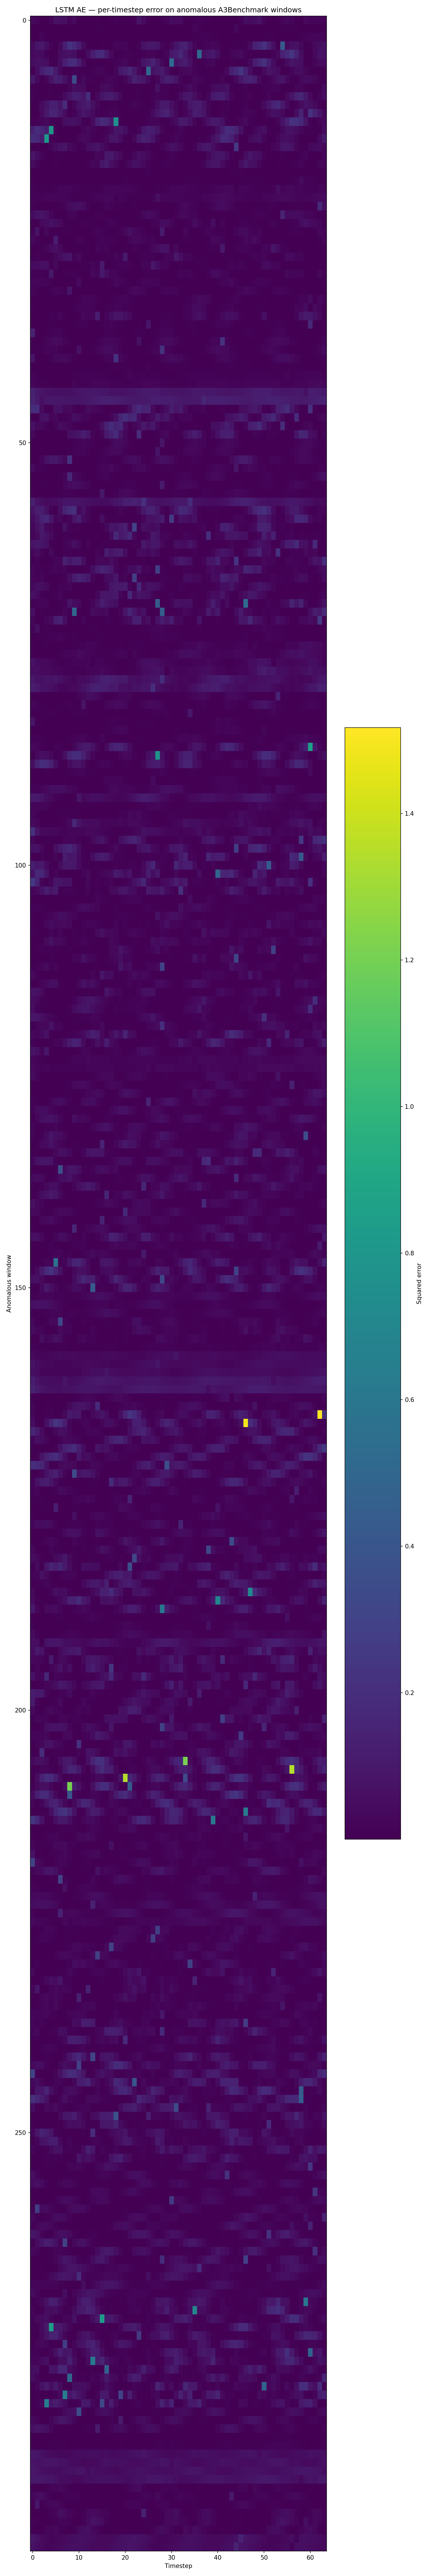
\includegraphics[height=0.55\textheight,keepaspectratio]{../../data/explainability/yahoo_A3Benchmark_lstm_vs_transformer/5/lstm_ae_error_heatmap.png}%
\hspace{0.04\textwidth}%
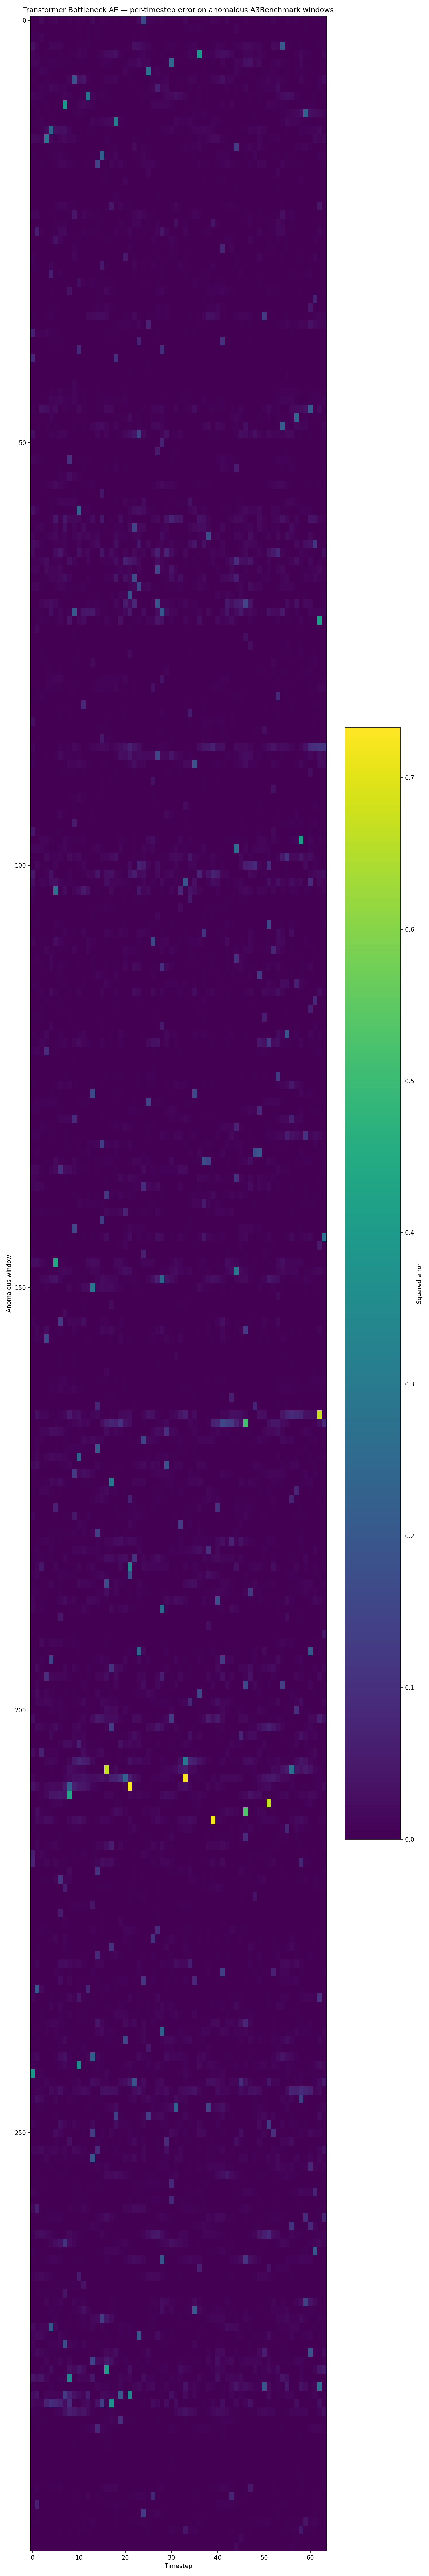
\includegraphics[height=0.55\textheight,keepaspectratio]{../../data/explainability/yahoo_A3Benchmark_lstm_vs_transformer/5/transformer_bottleneck_error_heatmap.png}

\caption{LSTM Autoencoder -- per-timestep squared reconstruction error on 300 randomly sampled anomalous A3 windows (one row per window, left). Elevated error appears as sparse, punctate points rather than as a uniform band, but a visibly larger share of rows carry a low-level elevated baseline across most of their width compared to the Transformer.}
\label{fig:explain-lstm-heatmap}
\caption{Transformer Bottleneck Autoencoder -- per-timestep squared reconstruction error on the same 300 anomalous A3 windows, same row order and colour scale convention as Figure~\ref{fig:explain-lstm-heatmap} (right). Error is visibly more sparse and confined to isolated timesteps.}
\label{fig:explain-transformer-heatmap}
\end{figure}

The visual comparison is broadly consistent with the initial assumption -- the Transformer's error concentrates into fewer, brighter points, while the LSTM Autoencoder's error is more often spread thinly across a window's full width -- but a heatmap read by eye is a weak instrument here: each panel is normalized to its own colour scale, and the LSTM Autoencoder's error values are roughly double the Transformer's in magnitude throughout, which alone would make its background look more saturated regardless of how concentrated the error actually is. A qualitative read of Figures~\ref{fig:explain-lstm-heatmap}--\ref{fig:explain-transformer-heatmap} therefore \emph{suggests} the phase-destruction mechanism but cannot confirm it.

\subsection{Quantitative Verification: Gini Coefficient of Error Concentration}

To separate genuine error concentration from an artifact of differing overall error magnitude, each anomalous window's 64 per-timestep squared errors were summarized with a Gini coefficient -- a standard inequality measure (originally used for income distributions) that is invariant to the absolute scale of its input. For a window's 64 error values sorted ascending, a Gini of 0 means the error is spread perfectly evenly across every timestep, and a Gini of 1 means it is concentrated entirely at a single timestep; unlike a raw magnitude comparison, this metric isolates the \emph{shape} of the error distribution within a window from its overall size.

For $n$ per-timestep squared errors $x_1 \le x_2 \le \dots \le x_n$ sorted ascending (here $n=64$), the Gini coefficient is computed as

\begin{equation}
G = \frac{2 \sum_{i=1}^{n} i \, x_i}{n \sum_{i=1}^{n} x_i} - \frac{n+1}{n}.
\label{eq:gini}
\end{equation}

Computed over the full population of 14{,}449 anomalous A3 windows, the two models separate clearly:

\begin{center}
\begin{tabular}{@{}lll@{}}
\toprule
 & Mean Gini & Median Gini \\
\midrule
LSTM Autoencoder & 0.566 & 0.606 \\
Transformer Bottleneck Autoencoder & 0.721 & 0.724 \\
\bottomrule
\end{tabular}
\end{center}

\begin{figure}[H]
\centering
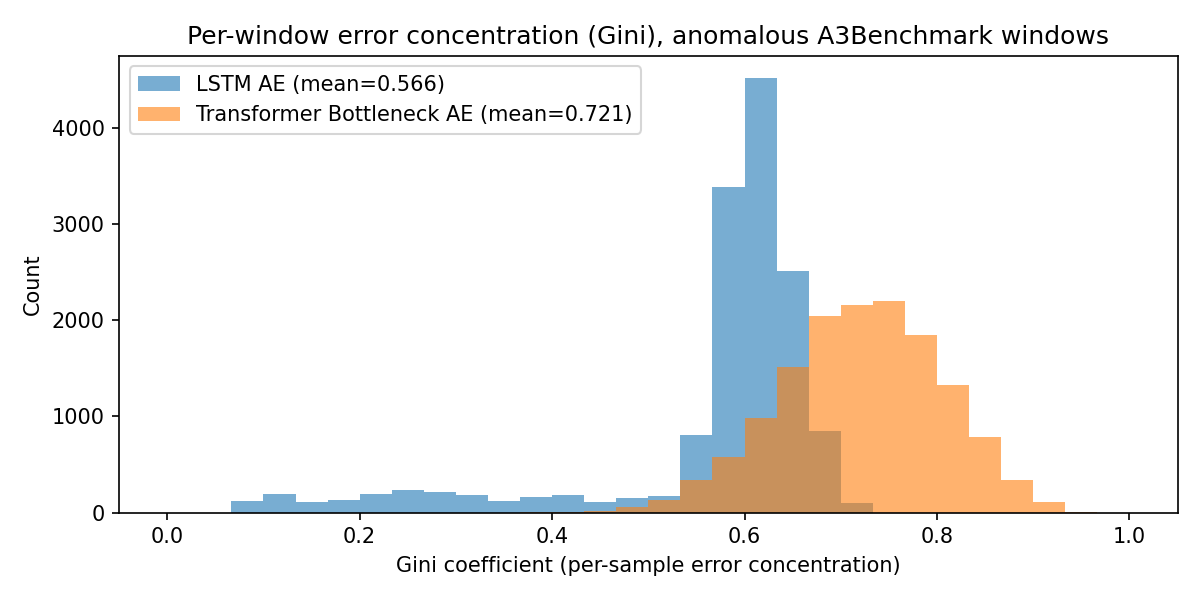
\includegraphics[width=0.7\textwidth]{../../data/explainability/yahoo_A3Benchmark_lstm_vs_transformer/5/gini_comparison.png}
\caption{Distribution of per-window Gini coefficients across all 14{,}449 anomalous A3 windows. The Transformer's distribution is unimodal and shifted toward high concentration (Gini $>0.6$); the LSTM Autoencoder's distribution is bimodal, with a majority clustered near the Transformer's range but a distinct secondary population spread across low Gini values (error genuinely smeared across the window).}
\label{fig:explain-gini}
\end{figure}

This confirms the initial assumption on average: the Transformer's error is more concentrated than the LSTM Autoencoder's across the full anomalous population, not merely in the handful of examples a heatmap happens to display. But the distribution in Figure~\ref{fig:explain-gini} reveals a detail the aggregate means alone would miss -- the LSTM Autoencoder's Gini values are \emph{bimodal}, not uniformly shifted down. A majority of its windows cluster in essentially the same high-concentration range as the Transformer's (Gini $\approx 0.6$, comparable localization ability), while a distinct secondary population of windows sits at low Gini ($<0.4$), where the error genuinely is smeared close to evenly across the full window. This indicates the phase-destruction mechanism is not a uniform property of every LSTM Autoencoder reconstruction, but a failure mode affecting a specific subset of windows -- and it is this subpopulation, not a general degradation across all anomalous windows, that is responsible for dragging the LSTM Autoencoder's aggregate AP and ROC-AUC below the Transformer's, since on the remaining majority of windows the two models localize error comparably well.

\section{Pseudo-Sequence Reconstruction Error on Credit Card Fraud}
\label{sec:explain-cc}

The Credit Card Discussion in Chapter~\ref{ch:results} argues that the three "temporal" architectures (Predictive LSTM, LSTM Autoencoder, Transformer Bottleneck Autoencoder) do not see a genuine sequence: each reshapes a row's 29 independent, decorrelated PCA features into an artificial sequence of 29 scalar steps, in whatever order the columns happen to appear in the source CSV. Predictive LSTM's poor performance (AP 0.519) is attributed directly to this -- "adjacent PCA components are orthogonal/decorrelated by construction, so there is no real next-step signal to learn." This section tests the reconstruction-based half of that claim (LSTM Autoencoder, Transformer Bottleneck Autoencoder) with the same per-position error diagnostic used in \S\ref{sec:explain-yahoo}.

\subsection{Initial Assumption}

If the 29 column positions genuinely carry no meaningful order, per-position reconstruction error on fraud samples should look like unstructured noise: no column should consistently accumulate more error than any other across the fraud population, for either model. A structured, repeated pattern -- specific columns lighting up across many fraud samples -- would complicate that picture and call for a follow-up explanation.

\subsection{Qualitative Check: Per-Feature-Position Error Heatmaps}

Both trained models were reconstructed on the full fraud test population (492 samples), and the per-column squared error was plotted as a heatmap (one row per sample, one column per of the 29 feature positions), with a random subsample of 300 fraud samples used to keep the rendered image legible. Figures~\ref{fig:explain-cc-lstm-heatmap} and~\ref{fig:explain-cc-transformer-heatmap} show the result.

\begin{figure}[H]
\centering
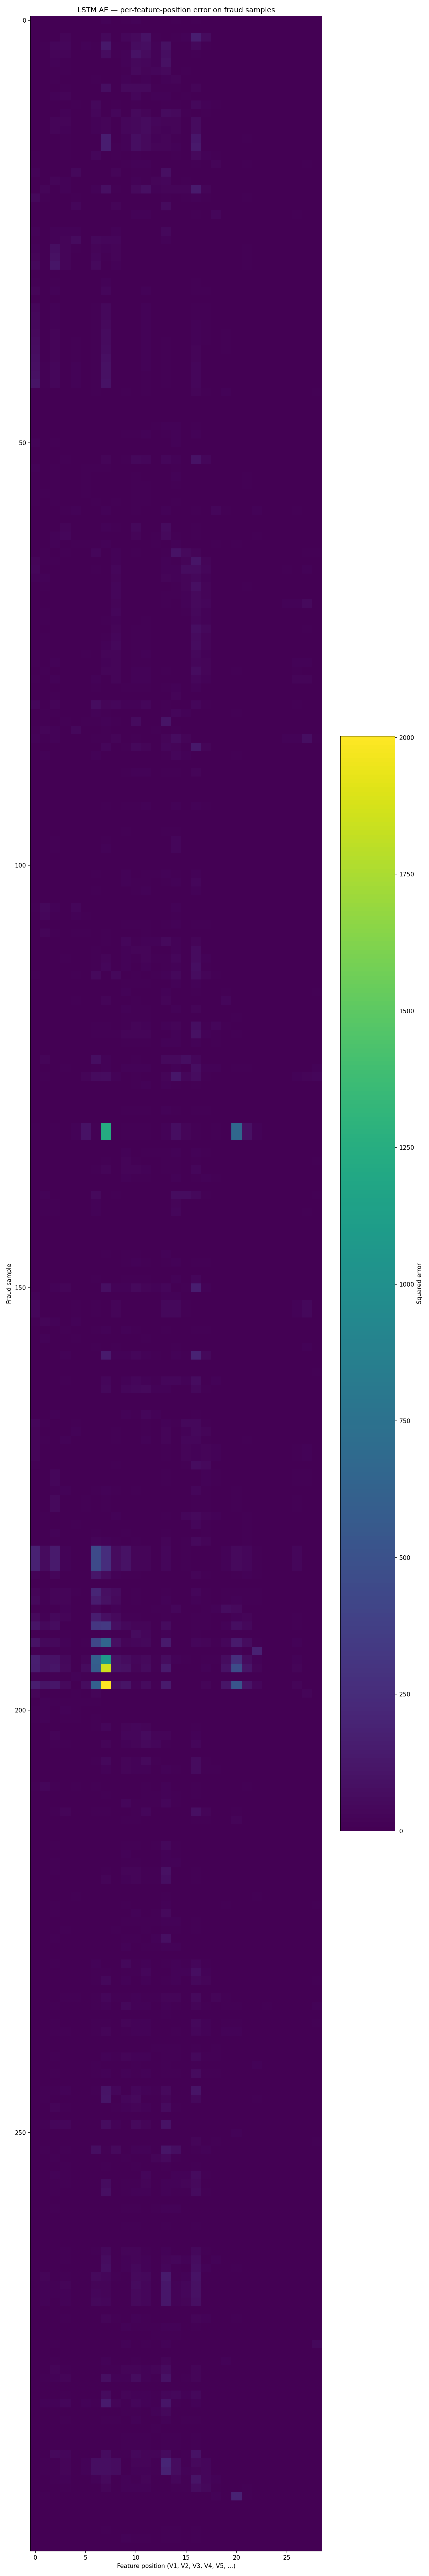
\includegraphics[height=0.55\textheight,keepaspectratio]{../../data/explainability/credit_card_lstm_vs_transformer/5/lstm_ae_error_heatmap.png}%
\hspace{0.04\textwidth}%
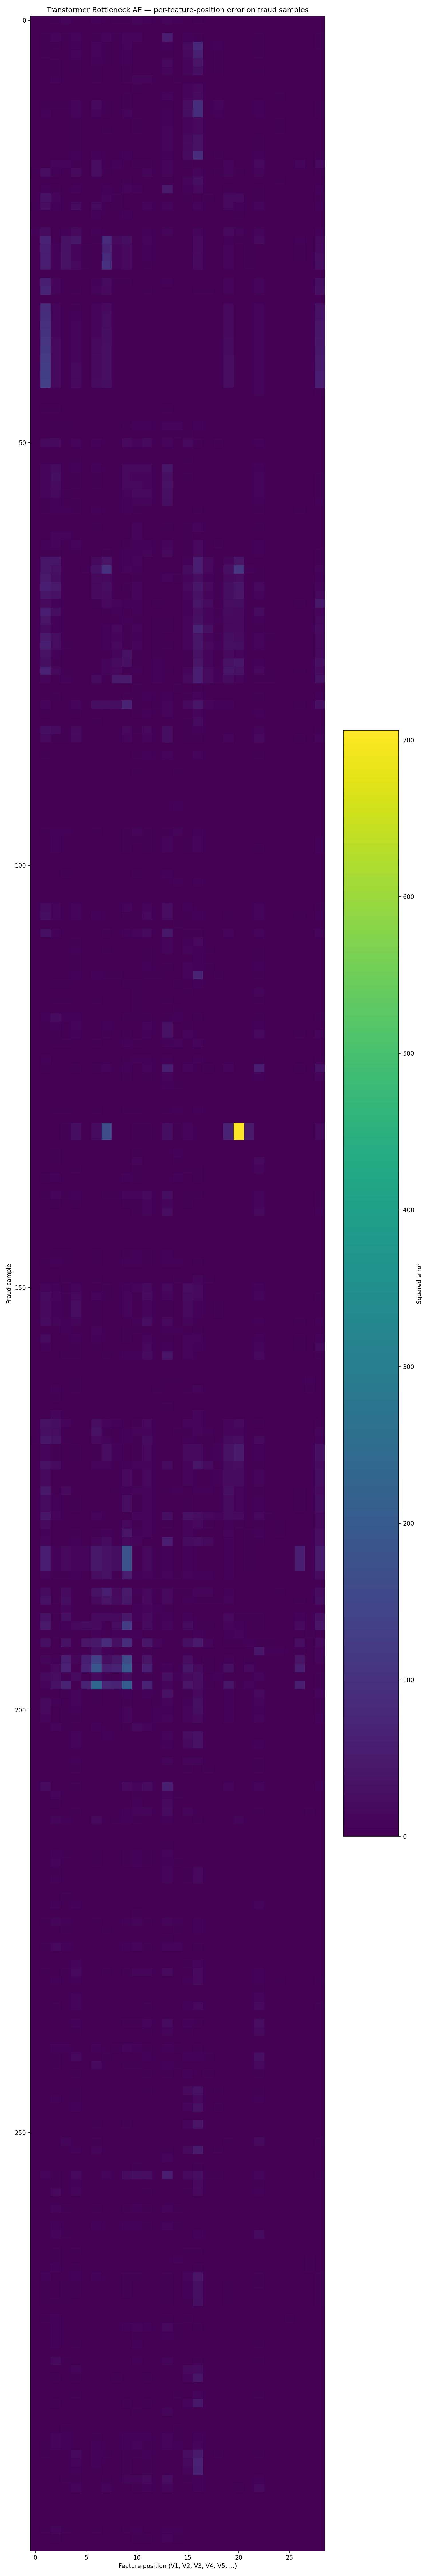
\includegraphics[height=0.55\textheight,keepaspectratio]{../../data/explainability/credit_card_lstm_vs_transformer/5/transformer_bottleneck_error_heatmap.png}

\caption{LSTM Autoencoder -- per-feature-position squared reconstruction error on 300 randomly sampled fraud transactions (one row per sample, columns V1--V28 then Amount, left).}
\label{fig:explain-cc-lstm-heatmap}
\caption{Transformer Bottleneck Autoencoder -- per-feature-position squared reconstruction error on the same 300 fraud transactions, same row order and column convention as Figure~\ref{fig:explain-cc-lstm-heatmap} (right).}
\label{fig:explain-cc-transformer-heatmap}
\end{figure}

Contrary to the initial assumption, both heatmaps show a visibly structured, repeated pattern: a handful of column positions accumulate elevated error across many fraud rows, rather than error being scattered evenly across all 29 positions. This does not by itself contradict the "no real sequence" claim -- it does not show that the models exploit \emph{order}, only that error is not uniformly distributed across \emph{columns}. Two distinct explanations are consistent with a structured heatmap: either specific PCA features are simply harder to reconstruct on fraud rows regardless of where they sit in the row (a feature-\emph{identity} effect, fully compatible with "no real sequence"), or the models are exploiting some incidental adjacency between specific neighbouring columns in this one fixed ordering (a position effect, which would nuance but not overturn the claim, since that adjacency is still arbitrary and non-causal). The heatmap alone cannot distinguish these.

\subsection{Quantitative Verification: Column-Shuffle Feature-Identity Check}

To separate the two explanations, the same 492 fraud rows were re-run through both models with a fixed random permutation of the 29 columns applied first (seed 42), and the per-column error was re-ranked. If the same underlying features dominate the top-error positions in both the original and the shuffled column order, the effect is feature-identity-driven; if overall error also changes substantially after shuffling, position/adjacency plays a role too.

\begin{center}
\resizebox{\textwidth}{!}{%
\begin{tabular}{@{}lccl@{}}
\toprule
 & Overlap (top 10, orig.\ vs.\ shuffled) & Top-error magnitude, orig.\ $\to$ shuffled & Stable top features (in both orderings) \\
\midrule
LSTM Autoencoder & 6/10 & 47.7 $\to$ 71.7 & V1, V3, V7, V8, V14, V17 \\
Transformer Bottleneck AE & 6/10 & 12.9 $\to$ 136.8 & V2, V3, V7, V8, V14, V17 \\
\bottomrule
\end{tabular}%
}
\end{center}

Both effects are present. Six of the top 10 highest-error features are the same before and after shuffling, for both models -- well above the $\sim$3--4 expected in common between two independent random top-10 draws out of 29 features under a pure-noise null. \textbf{V14 and V17 are stable top accumulators for both models under both orderings}, and both are independently singled out by the community exploratory notebook cited in Chapter~\ref{ch:methodology} as its two strongest negative correlates with the fraud label -- an external check that these two features genuinely carry fraud-relevant signal, not an artifact of this experiment. At the same time, overall error rose substantially after shuffling for both models (LSTM Autoencoder's top value: 47.7 $\to$ 71.7; Transformer's: 12.9 $\to$ 136.8), which only makes sense if both encoders were also leaning on some incidental adjacency between specific neighbouring columns in the fixed, original CSV order.

Taken together, this confirms the core claim with a refinement the aggregate metrics could not surface on their own: the reconstruction-based architectures did learn to depend on the one fixed, arbitrary column ordering supplied at preprocessing time, beyond what a pure feature-identity effect would predict. The fact that error went up means the models had implicitly learned something that depended on which value sat next to which in the specific column arrangement the CSV happens to use, even though that adjacency is meaningless (it's just PCA-component arbitrary order)
 - not evidence of a hidden causal sequence in the data, but more like the models overfit to an arbitrary but fixed layout

\section{Disjoint Feature Regimes: AE+Context vs.\ Temporal IForest}
\label{sec:explain-disjoint-regime}

The CIC-IDS2017 Discussion in Chapter~\ref{ch:results} proposes pairing AE+Context (strong on DDoS and PortScan) with Temporal IForest (strong on the slow-DoS classes and, tentatively, Heartbleed) into a practical ensemble, since the two operate on disjoint feature regimes -- host-context features versus a 16-flow temporal window. That argument rests on two separate premises, one per model: that Temporal IForest's score is genuinely informed by the window's temporal structure rather than by one flow's static feature values sitting inside a wider, functionally inert vector; and that AE+Context's score is genuinely informed by the host-context features unique to it, rather than by the same flow-level features Temporal IForest already has access to. Both are tested in turn below.

\subsection{Temporal IForest: Initial Assumption}

If Temporal IForest is genuinely exploiting cross-timestep structure, its per-window score should remain informative about the \emph{last} flow's own label -- the flow that would be paired with AE+Context's per-flow score in the ensemble -- rather than only about whether \emph{some} flow within the 16-flow window is an attack. Its SHAP attribution should also not collapse onto that single last flow; if it does, the window is decorative and the ``disjoint feature regime'' argument for the ensemble does not hold.

\subsection{Temporal IForest: Score Validity Under Last-Flow Labeling}

The originally showed per-class AP figures use an ``any-of-16'' window label: a window is positive if any of its 16 flows is an attack, tagged with the majority attack type. That is more lenient than the per-flow labeling AE+Context is scored against. Every existing test window was relabeled by its \emph{last} flow's own true label instead, and per-class AP recomputed against the unchanged, already-trained model and its existing scores.

\begin{center}
\begin{tabular}{@{}lccc@{}}
\toprule
 & AP (any-of-16) & AP (last-flow) & $n$ (last-flow) \\
\midrule
DDoS              & 0.9518 & 0.9515 & 95{,}123 \\
DoS GoldenEye     & 0.6278 & 0.6265 & 7{,}567 \\
DoS Slowhttptest  & 0.6851 & 0.6849 & 1{,}742 \\
DoS slowloris     & 0.6091 & 0.6077 & 4{,}001 \\
Heartbleed        & 0.5927 & 0.2892 & 11 \\
\bottomrule
\end{tabular}
\end{center}

We see AP is essentially unchanged for all four target classes under the stricter labeling, confirming the score is informative about the last flow's own status, not an artifact of the lenient window label. Heartbleed drops sharply, but on only 11 true flows -- its entire test population -- so it is excluded from the ensemble and treated as tentative, consistent with its hedged treatment in Chapter~\ref{ch:results}.

\subsection{Temporal IForest: SHAP Attribution Across the Window}
\label{sec:explain-temporal-window}

Temporal IForest is trained on flattened 16-flow windows, so \texttt{TreeExplainer}'s SHAP values on the flattened input decompose cleanly back into a (window, timestep, feature) cube. For each of the four classes, SHAP was computed on 200 windows; attribution magnitude was summed over features per timestep to check for concentration on the final timestep, and the top contributing features were plotted across all 16 timesteps to check whether the same feature carries consistent-sign attribution throughout the window rather than only near the end.

\begin{figure}[H]
\centering
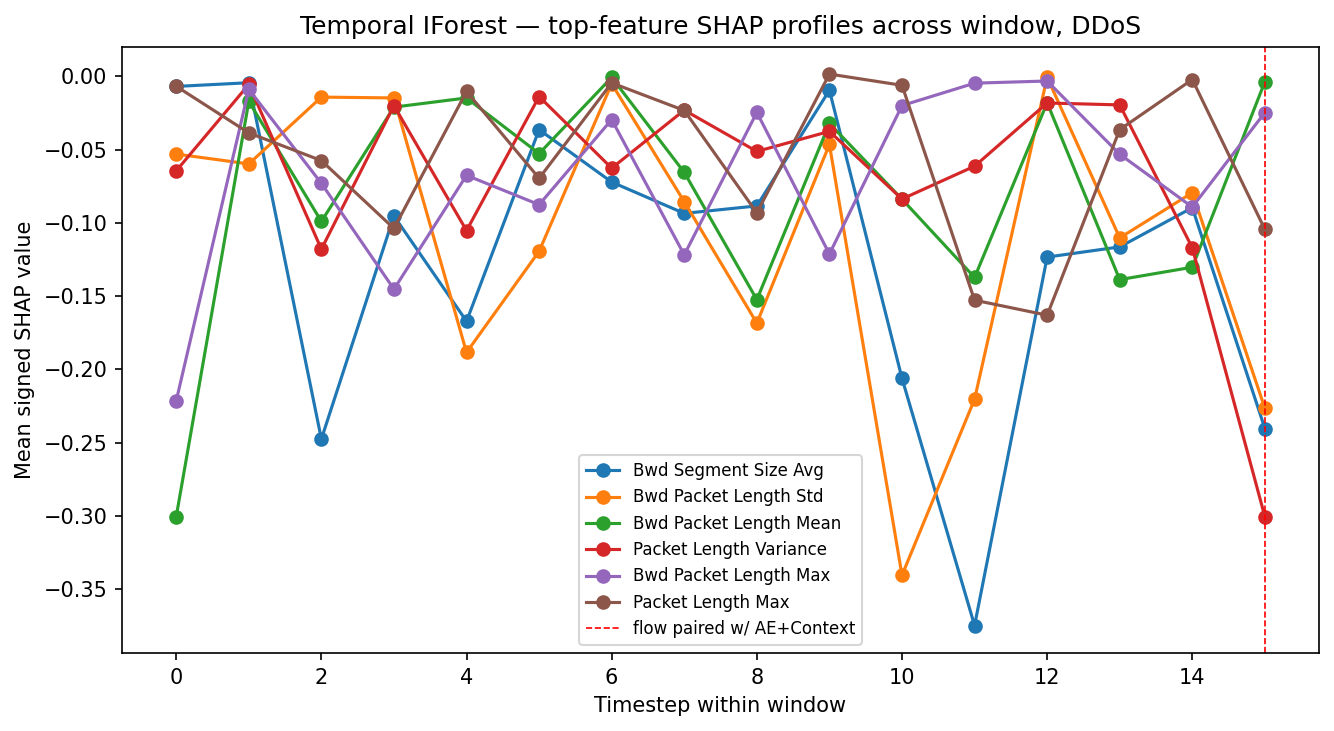
\includegraphics[width=0.48\textwidth,keepaspectratio]{../../data/explainability/cicids_temporal_shap/1/ddos_top_feature_profiles.png}%
\hspace{0.02\textwidth}%
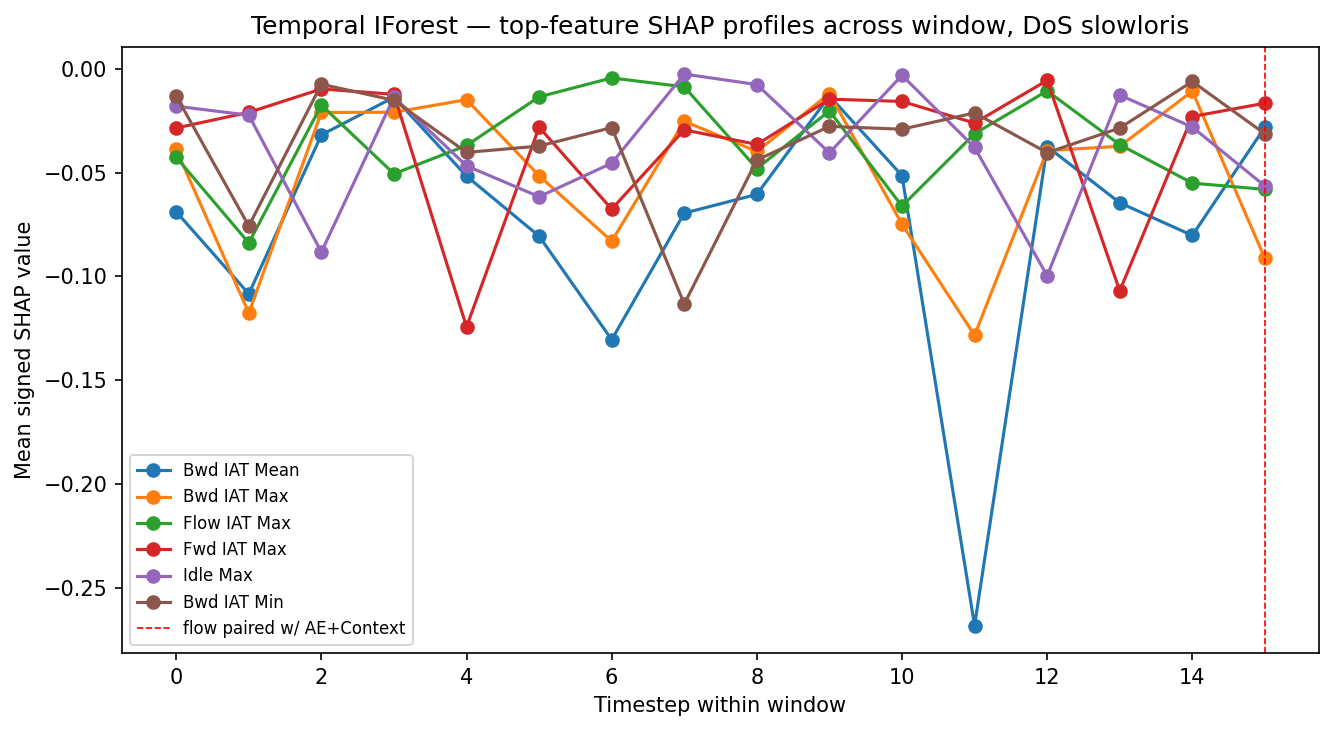
\includegraphics[width=0.48\textwidth,keepaspectratio]{../../data/explainability/cicids_temporal_shap/1/dos_slowloris_top_feature_profiles.png}

\caption{Temporal IForest -- mean SHAP value per timestep for the six most-attributed features, DDoS windows (left) and DoS slowloris windows (right). In both cases attribution is negative (anomalous), recurs at consistent sign across most of the 16 timesteps, and does not concentrate at the final flow (dashed red line) -- the flow paired with AE+Context's score in the proposed ensemble.}
\label{fig:explain-temporal-shap}
\end{figure}

\begin{figure}[H]
\centering
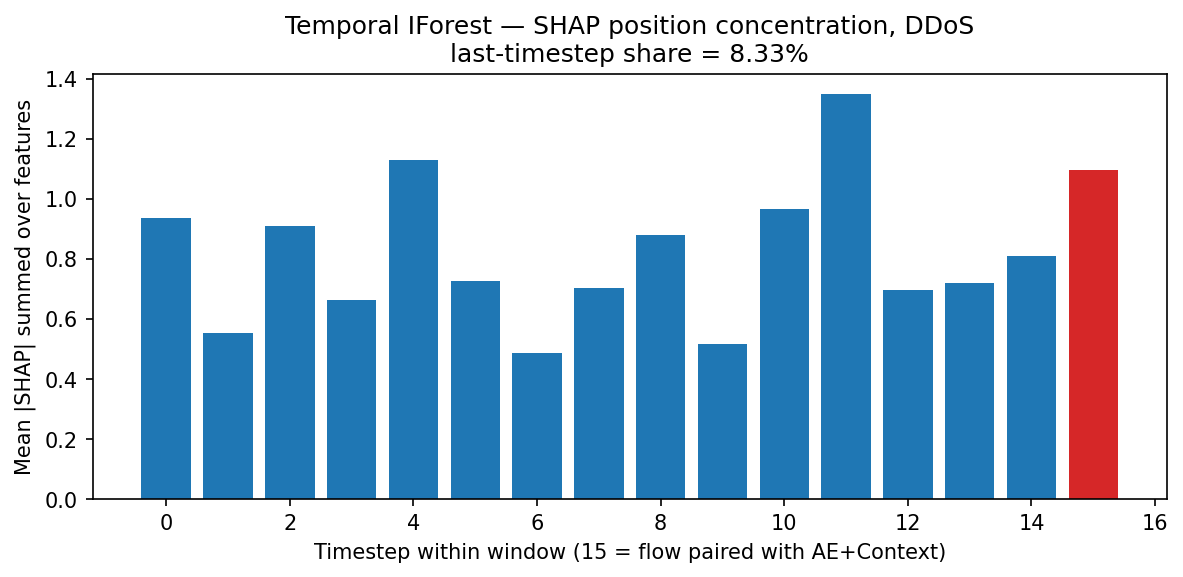
\includegraphics[width=0.48\textwidth,keepaspectratio]{../../data/explainability/cicids_temporal_shap/2/ddos_position_concentration.png}%
\hspace{0.02\textwidth}%
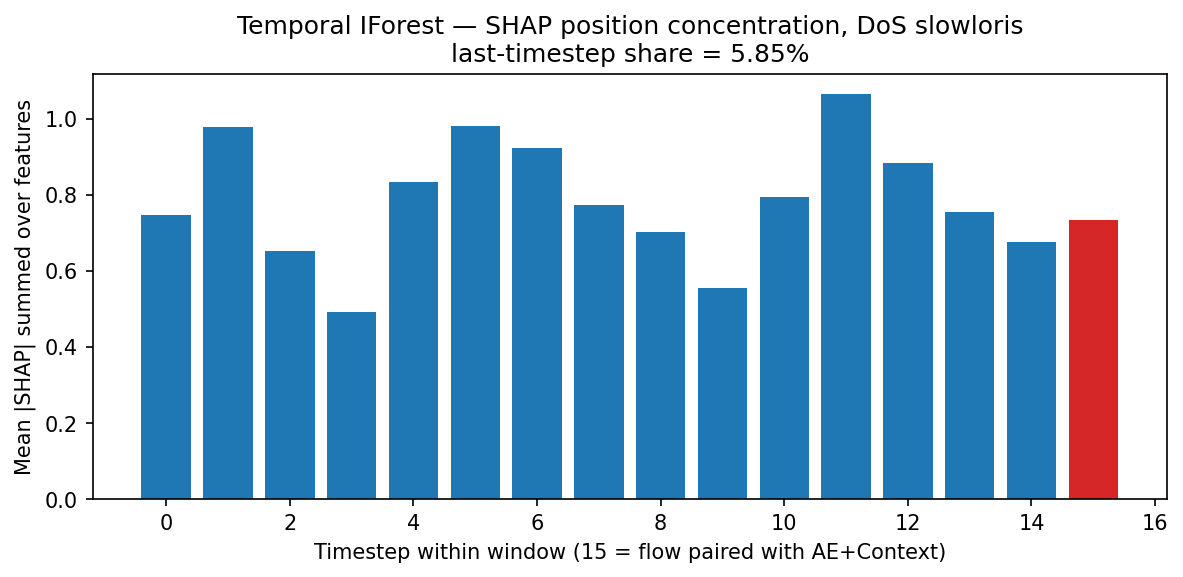
\includegraphics[width=0.48\textwidth,keepaspectratio]{../../data/explainability/cicids_temporal_shap/2/dos_slowloris_position_concentration.png}
\caption{Temporal IForest -- mean $|\text{SHAP}|$ summed over features, per timestep, DDoS windows (left) and DoS slowloris windows (right). The final timestep (red bar, 15) -- the flow paired with AE+Context's score in the proposed ensemble -- carries no more attribution mass than any other position in the window, confirming the summary statistic reported below.}
\label{fig:explain-temporal-position-concentration}
\end{figure}

\begin{figure}[H]
\centering
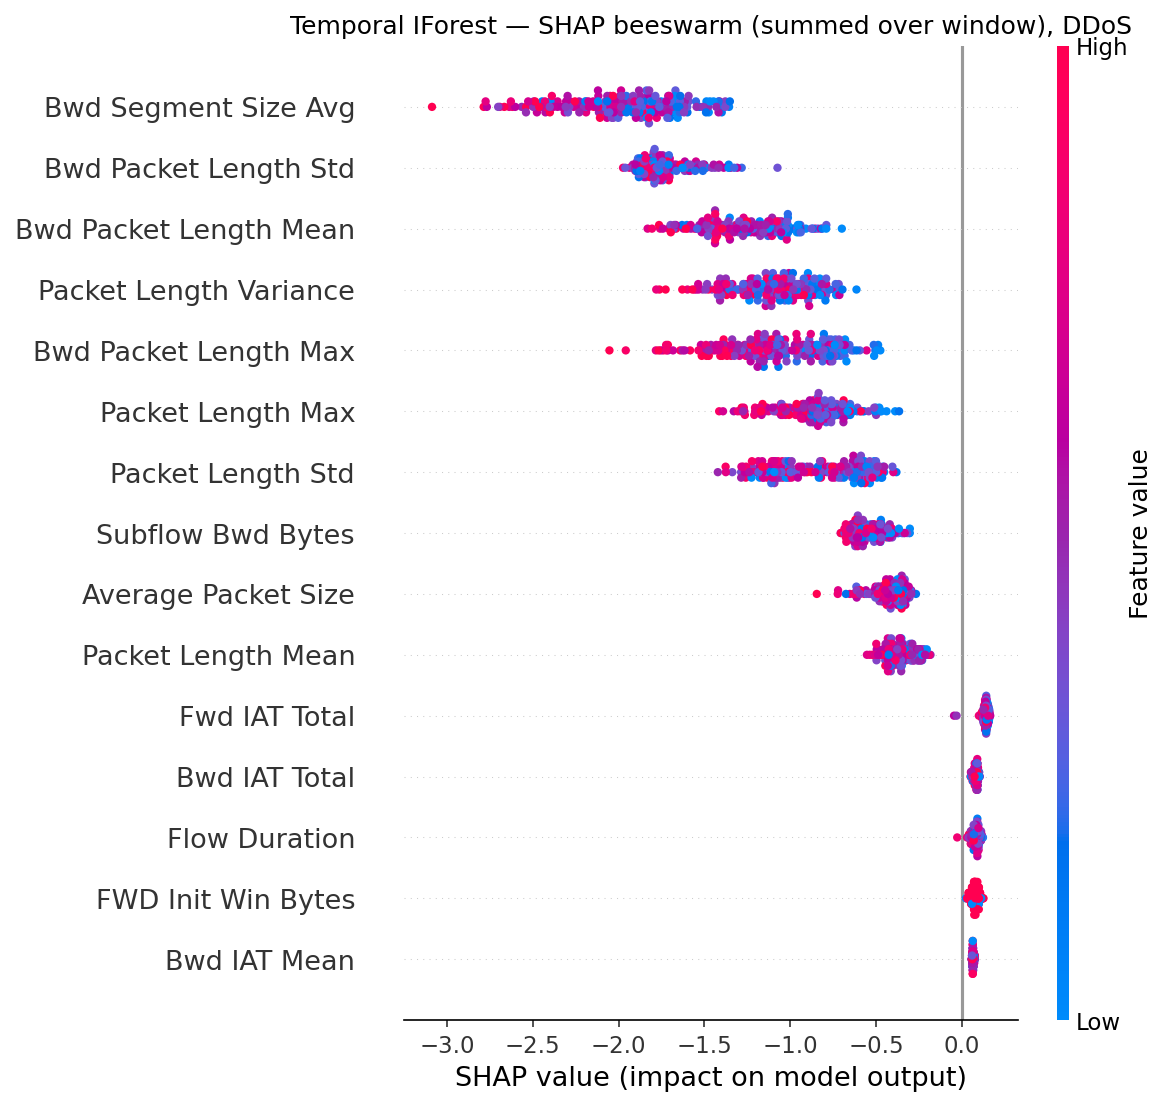
\includegraphics[width=0.48\textwidth,keepaspectratio]{../../data/explainability/cicids_temporal_shap/2/ddos_beeswarm.png}%
\hspace{0.02\textwidth}%
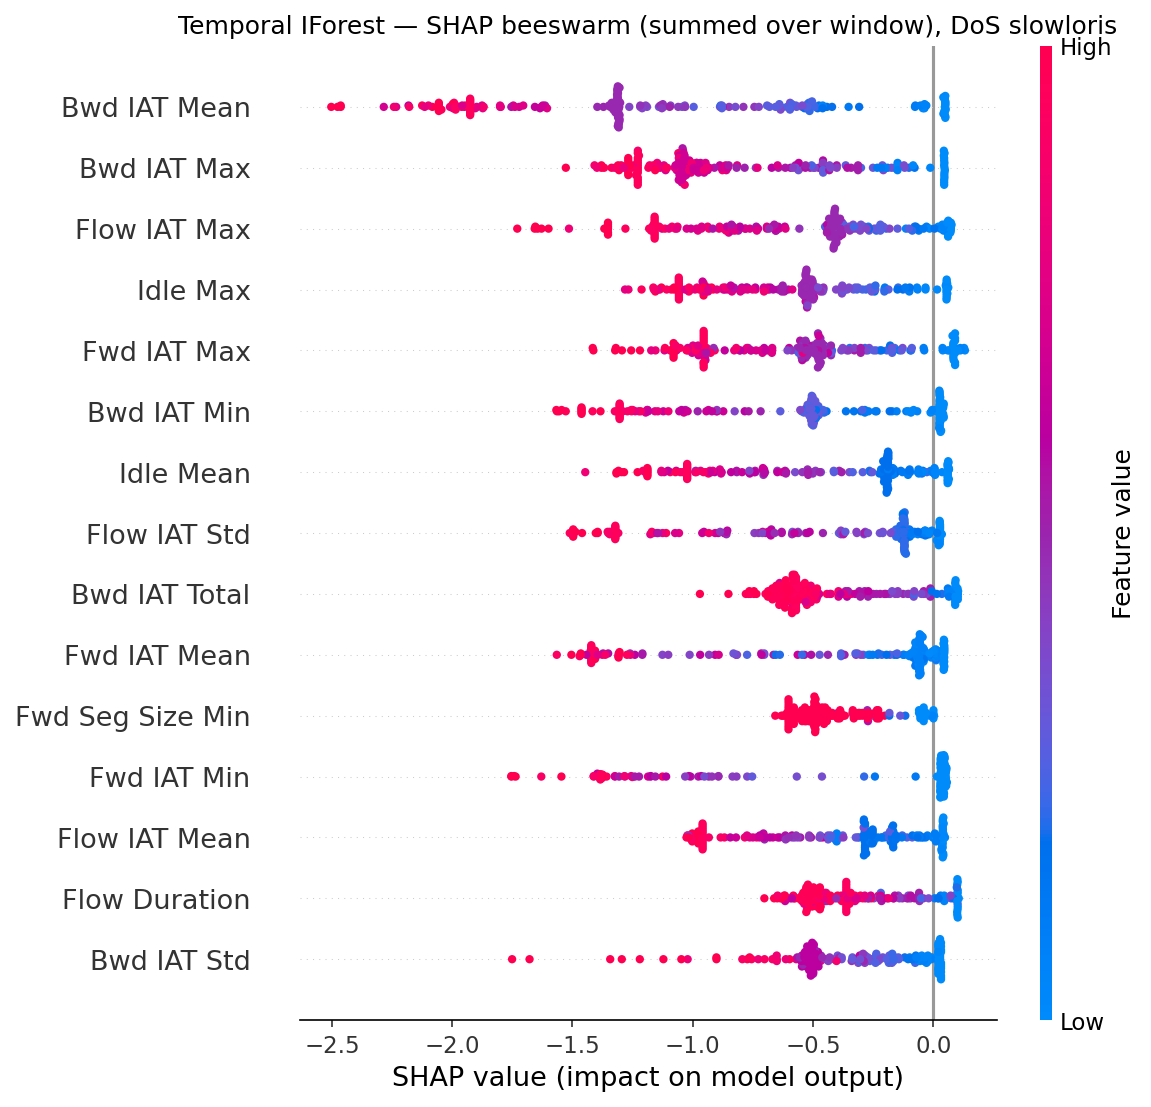
\includegraphics[width=0.48\textwidth,keepaspectratio]{../../data/explainability/cicids_temporal_shap/2/dos_slowloris_beeswarm.png}
\caption{Temporal IForest -- SHAP beeswarm per feature, DDoS windows (left) and DoS slowloris windows (right), collapsing the 16-timestep axis by summing each feature's SHAP contribution across the window and coloring by that feature's mean value across the window. DoS slowloris shows a clean monotonic relationship -- high inter-arrival-time values drive strongly negative (anomalous) SHAP, low values push near zero -- consistent with the slow, connection-holding behaviour the attack is named for. DDoS shows a noisier value-to-sign relationship for its backward-packet-length features, and a wider per-window spread than the mean-only view in Figure~\ref{fig:explain-temporal-shap} suggests on its own.}
\label{fig:explain-temporal-beeswarm}
\end{figure}

The final timestep -- the one paired with AE+Context in the ensemble -- carries only 6--8\% of total attribution mass across all four classes, close to the 6.25\% uniform baseline for a 16-step window, rather than dominating it. The top features also match each attack's known mechanism: DDoS and DoS GoldenEye attribution concentrates on backward-packet-length statistics (\texttt{Bwd Packet Length Std/Mean/Max}, \texttt{Packet Length Variance}), consistent with a volumetric flood; DoS Slowhttptest and DoS slowloris attribution concentrates on inter-arrival-time statistics (\texttt{Fwd/Bwd IAT Std/Max}, \texttt{Idle Mean/Max}), consistent with the slow, connection-holding behaviour these attacks are named for. This confirms the initial assumption: Temporal IForest's advantage on these classes reflects genuinely disjoint temporal evidence, not a relabeled copy of one flow's static features -- supporting the ``disjoint feature regime'' premise behind pairing it with AE+Context.

\subsection{AE+Context: SHAP Dominated by Host-Context Features}

The mirror premise is that AE+Context's advantage on its own strong classes -- DDoS and PortScan, per Chapter~\ref{ch:results} -- traces to the 9 \texttt{ctx\_*} host-context features unique to its feature set, rather than to the same flow-level features Temporal IForest already sees. If instead AE+Context's attribution spreads across ordinary flow features, its complementarity with Temporal IForest would be coincidental rather than a genuinely disjoint evidence source.

SHAP was computed with \texttt{GradientExplainer} on AE+Context's reconstruction error, on 200 samples each of PortScan and DDoS, and the 15 features with the highest mean $|\text{SHAP}|$ were ranked for each class.

\begin{figure}[H]
\centering
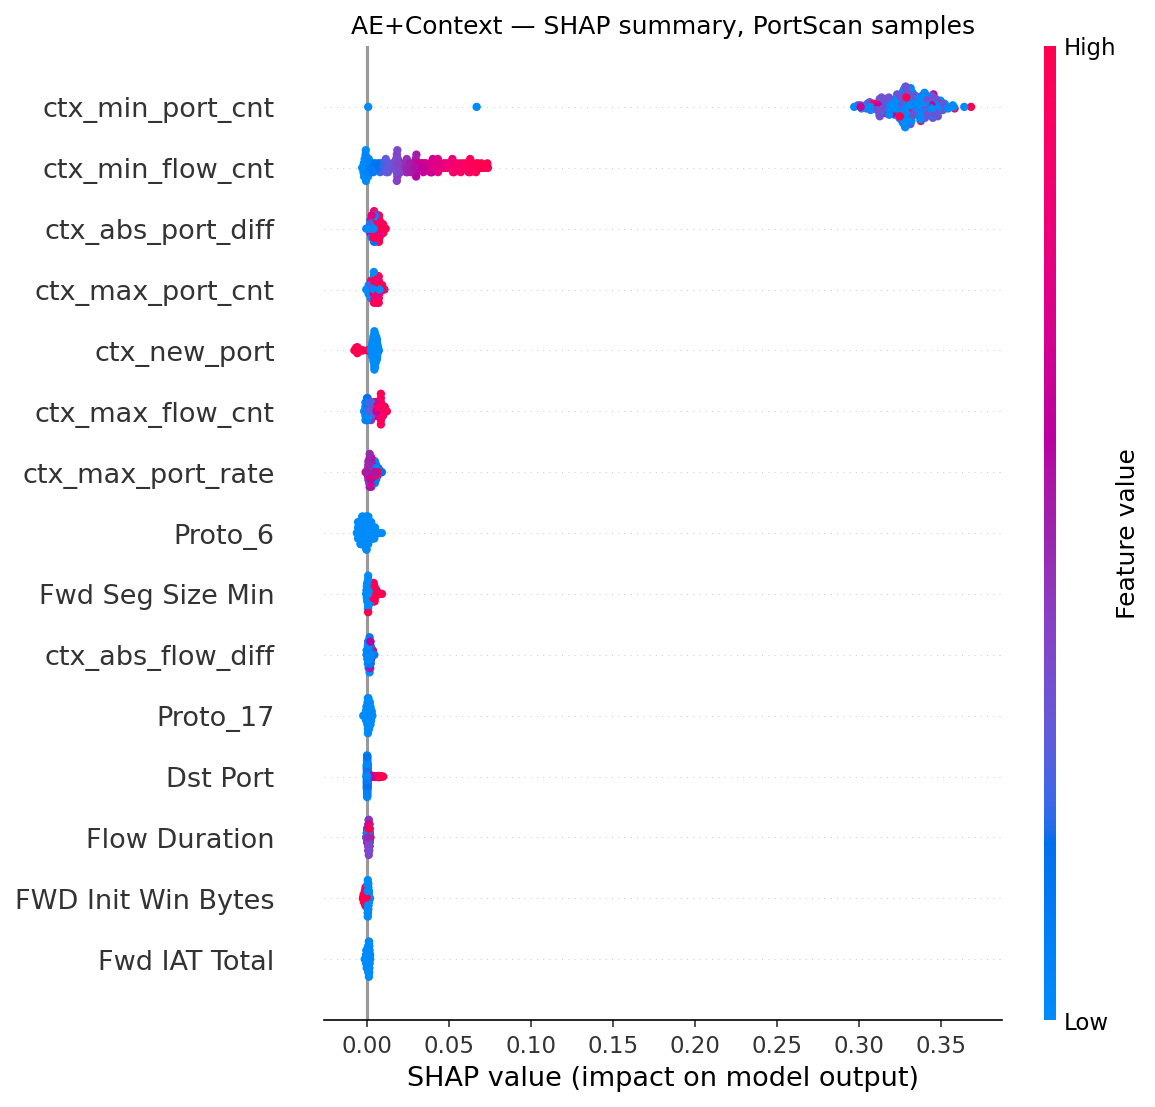
\includegraphics[width=0.75\textwidth]{../../data/explainability/cicids_shap_portscan/5/autoencoder_context_portscan_shap.png}
\caption{AE+Context -- SHAP summary plot, PortScan samples. \texttt{ctx\_min\_port\_cnt} dominates with a tight, uniformly positive-SHAP cluster well separated from every other feature; the remaining top rows are almost entirely \texttt{ctx\_*} host-context features, with ordinary flow features only appearing near the bottom of the ranking.}
\label{fig:explain-ae-context-portscan-shap}
\end{figure}

\begin{center}
\begin{tabular}{@{}lcc@{}}
\toprule
 & \texttt{ctx\_*} features in top 15 & Leading feature (mean $|\text{SHAP}|$) \\
\midrule
PortScan & 8/15 & \texttt{ctx\_min\_port\_cnt} (0.324) \\
DDoS     & 7/15 & \texttt{ctx\_min\_port\_cnt} (0.234) \\
\bottomrule
\end{tabular}
\end{center}

For both classes, \texttt{ctx\_min\_port\_cnt} and \texttt{ctx\_min\_flow\_cnt} dominate by roughly an order of magnitude over every ordinary flow feature: on PortScan, \texttt{ctx\_min\_port\_cnt}'s attribution (0.324) is nearly 70$\times$ the next-highest ordinary feature, \texttt{Fwd Seg Size Min} (0.0023); on DDoS it is over 6$\times$ the leading ordinary feature, \texttt{Bwd Packet Length Std} (0.035). Six of the nine \texttt{ctx\_*} features appear in both classes' top-15 lists, with only \texttt{ctx\_min\_port\_rate} absent from both. This confirms the mirror premise: AE+Context's advantage on these classes is driven almost entirely by host-context evidence unavailable to Temporal IForest, not by the ordinary flow features the two models share.

Taken together with \S\ref{sec:explain-temporal-window}'s result for Temporal IForest, the two halves of the disjoint-feature-regime premise both hold: Temporal IForest's strong classes are explained by evidence spread across the 16-flow window (packet-length statistics for volumetric floods, inter-arrival-time statistics for slow-drip attacks), and AE+Context's strong classes are explained by host-context features that exist only in its own feature set. The proposed ensemble's complementary coverage is therefore backed by genuinely non-overlapping evidence between its two members, not by two rankings that merely happen to differ on which classes they cover.

\subsection{Building the Combined Score}
\label{sec:explain-ensemble-build}

Confirming the disjoint-evidence premise does not by itself establish that combining the two scores works in practice. Realizing the ensemble sketched in Chapter~\ref{ch:results} requires pairing, for every flow $f$ in the test set, AE+Context's own per-flow score $s_{AE}(f)$ with Temporal IForest's score for the 16-flow window \emph{ending} at $f$ -- the same causal, non-leaking choice validated in the previous subsection via last-flow labeling. Since the two preprocessing pipelines reorder flows differently before saving their respective test arrays (AE+Context sorts globally by timestamp; Temporal IForest sorts per source-IP host), the two score arrays are not aligned index-for-index and must be re-aligned by flow identity, recovering each flow's original row position in both pipelines' shared, pre-sort input.

Once aligned, the two raw scores cannot be combined directly: AE+Context's score is a mean-squared reconstruction error with no fixed scale, and Temporal IForest's score is a negated mean path length, and the two live on entirely different numeric ranges. Some normalization is required before either a weighted average or a max can be meaningful. Each model's normalization statistics are computed on that same model's own \emph{benign training} scores only, never on test data, to avoid leaking test-set anomaly information into the fusion.

\subsection{Two Fusion Rules, Two Normalizations}
\label{sec:explain-ensemble-fusion}

Two combination rules were tested. \textbf{Weighted soft voting} takes a convex combination of the two normalized scores, $s_{\text{soft}}(f) = w \cdot \hat{s}_{AE}(f) + (1-w) \cdot \hat{s}_{IF}(f)$, swept over $w \in \{0.3, \dots, 0.7\}$. \textbf{Max-rule fusion} instead takes $s_{\text{max}}(f) = \max(\hat{s}_{AE}(f), \hat{s}_{IF}(f))$ -- an OR-like combiner intended to match the disjoint-evidence story more directly: either model's confidence alone should be enough to flag a flow.

The first normalization attempted, standard $z$-scoring against each model's own benign training mean and standard deviation, turned out to be a dead end rather than a genuine test of either fusion rule. AE+Context's reconstruction-error $z$-scores are extremely heavy-tailed (maximum $z \approx 2366$ on the test set, with the 99.9th percentile of \emph{benign} flows alone already at $z \approx 227$), while Temporal IForest's $z$-scores stay tightly bounded (maximum $z \approx 21$). Under $z$-score normalization, a handful of extreme AE+Context outliers dominate any linear combination or max regardless of the weight assigned to Temporal IForest: max-rule and every soft-vote weight tested reproduced AE+Context's own per-class ranking almost exactly (e.g.\ GoldenEye AP stayed at $0.215$--$0.216$ across all five weights, against AE+Context alone's $0.215$), rather than showing any influence from Temporal IForest's much stronger $0.627$ standalone score on that class. This is a normalization artifact, not evidence that fusion does not help -- it does not actually test the ensemble hypothesis.

Replacing $z$-score with rank normalization -- mapping each test score to its percentile within that model's own benign training-score distribution, via the empirical CDF -- removes this problem by construction: every normalized score is bounded to $[0,1]$ regardless of how extreme the raw value is, so neither model's tail can dominate the other's by sheer magnitude. All results below use rank normalization.

\subsection{Per-Class Coverage vs.\ Aggregate AP}
\label{sec:explain-ensemble-results}

\begin{center}
\begin{tabular}{@{}lccccc@{}}
\toprule
 & DDoS & PortScan & GoldenEye & Slowhttptest & slowloris \\
\midrule
AE+Context alone        & 0.882 & \textbf{0.924} & 0.292 & 0.013 & 0.025 \\
Temporal IForest alone  & \textbf{0.956} & 0.123 & 0.611 & 0.578 & 0.560 \\
Max-rule (rank)         & 0.882 & 0.923 & 0.292 & 0.060 & 0.083 \\
Soft-vote $w=0.4$ (rank) & 0.977 & 0.228 & \textbf{0.801} & \textbf{0.205} & \textbf{0.319} \\
Soft-vote $w=0.7$ (rank) & 0.977 & 0.358 & 0.821 & 0.140 & 0.245 \\
\bottomrule
\end{tabular}
\end{center}

Aggregate AP over the full row-aligned test set actually \emph{favors} the variants that change the least: max-rule (aggregate AP $0.943$) and AE+Context alone ($0.941$) both edge out soft-vote $w=0.4$ ($0.841$), simply because DDoS and PortScan together account for over 250{,}000 of the roughly 434{,}000 positive flows in this evaluation, while GoldenEye, Slowhttptest, and slowloris combined account for barely 13{,}000. An aggregate metric dominated by two classes' raw volume is exactly the wrong lens for judging whether an ensemble motivated by \emph{per-class coverage} actually delivers it, so \S\ref{sec:cic-per-attack}'s per-class breakdown, not the aggregate table, is the right basis for evaluating this ensemble -- consistent with how every other per-attack-type claim in this thesis is judged.

Read per-class, max-rule falls short of its own premise: because it is an OR over two scores, it inherits the \emph{union} of both models' false-positive tendencies rather than only their true positives, so on GoldenEye/Slowhttptest/slowloris it barely moves off AE+Context's own weak scores ($0.292 \to 0.292$, $0.013 \to 0.060$, $0.025 \to 0.083$) despite Temporal IForest's much stronger standalone numbers on exactly these classes. Soft voting shows the opposite failure mode on PortScan: because it averages rather than maxes, and Temporal IForest is actively poor on PortScan ($0.123$, well below AE+Context's $0.924$) rather than merely uninformative, blending pulls PortScan's ranking down substantially ($0.924 \to 0.228$ at $w=0.4$) even while lifting GoldenEye from $0.292$ to $0.801$.

Neither rule is a free win, but soft voting is the more defensible choice for a coverage-motivated ensemble: its \emph{weakest} covered class ($0.205$, Slowhttptest, at $w=0.4$) clears both standalone models' own weakest classes -- AE+Context's $0.013$ (Slowhttptest) and Temporal IForest's $0.123$ (PortScan) -- something neither standalone model nor max-rule fusion achieves. This is a genuine, if partial, realization of the ensemble idea from Chapter~\ref{ch:results}: rank-normalized soft voting measurably widens the floor of attack-class coverage, at the explicit cost of PortScan detection quality, rather than the free lunch the original aggregate-level framing implied. A deployment that must retain AE+Context's near-complete PortScan coverage would instead need a class-aware combination rule (e.g.\ routing PortScan-like flows to AE+Context alone) rather than a single global weight -- left as future work.

\chapter{Concluzii}
\label{ch:concluzii}

Întrebarea formulată în Capitolul~\ref{ch:introducere} a fost în ce măsură modul în care un model reprezintă structura latentă a datelor \enquote{normale} determină tipurile de anomalii pe care le poate detecta. Rezultatele din Capitolul~\ref{ch:results}, confirmate și nuanțate în Capitolul~\ref{ch:explainability}, dau un răspuns afirmativ: aceeași paradigmă produce rezultate diferite pe seturi de date diferite, nu pentru că modelul ar fi mai bun sau mai slab în sine, ci pentru că presupunerea lui despre normalitate se potrivește sau nu structurii reale a anomaliei căutate.

Cât despre cele două ipoteze formulate în \S\ref{sec:expected-behaviour}, ele se confirmă, dar nu necondiționat. Prima ipoteză -- că structura temporală inerentă avantajează seturile de date cu adevărat secvențiale -- se confirmă clar pe Yahoo A3/A4, unde paradigma predictivă domină, dar se inversează pe Setul de Date A (unde secvența este artificială) și este depășită de caracteristicile de context la CIC-IDS2017, unde reconstrucția câștigă în ciuda structurii temporale disponibile.\
A doua ipoteză -- că paradigme complementare, combinate într-un ansamblu, îmbunătățesc performanța -- este confirmată de studiul de caz din \S\ref{sec:explain-disjoint-regime}: AE+Context și Temporal IForest exploatează, demonstrabil prin SHAP, evidențe disjuncte, iar votarea ponderată extinde acoperirea pe clase de atac pe care niciun model singur nu le detectează bine. Câștigul nu este însă gratuit -- vine cu un cost pe AP-ul agregat, dominat de clasele majoritare -- ceea ce nuanțează, mai degrabă decât infirmă, ipoteza inițială.

Limitările acestei lucrări deschid două direcții clare de continuare: testarea sistematică a celorlalte presupuneri ridicate în discuțiile Capitolului~\ref{ch:results} -- de exemplu de ce ferestrele temporale dăunează performanței la Setul de Date A și C, sau de ce clase precum FTP-Patator, SSH-Patator, Bot rămân nedetectabile indiferent de setul de caracteristici; și extinderea studiului de ansamblu din \S\ref{sec:explain-ensemble-build} la Setul de Date A și B, cu reguli de combinare mai sofisticate decât votarea ponderată și regula maximului.

\enlargethispage{\baselineskip}

\appendix
\chapter{Alegeri legate de Hiperparametri și Antrenare}
\label{sec:architecture}

Două decizii principale se aplică uniform pentru toate modelele și seturile de date:

\begin{itemize}
  \item \textbf{Optimizator.} Toate rețelele neuronale sunt antrenate cu Adam, la o rată de învățare fixă de $10^{-3}$, uniform pentru fiecare model și set de date.
  \item \textbf{Fără căutare de hiperparametri.} Dacă un model a avut performanțe neașteptat de slabe, rata sa de învățare a fost verificată suplimentar cu $\{10^{-4}, 10^{-3}, 3\times10^{-3}\}$ înainte de a trage vreo concluzie din acel rezultat.
  \item \textbf{Partiție de validare doar pentru monitorizare.} Fiecare rețea neuronală reține aleator 10\% din datele de antrenare exclusiv pentru a trasa o curbă de pierdere (\emph{loss}) de antrenare/validare per rulare, ca verificare că antrenarea decurge corect. Această partiție nu este niciodată folosită pentru oprire timpurie (\emph{early stopping}) sau selecția modelului: antrenarea rulează întotdeauna pentru numărul fix de epoci de mai jos, iar rezultatele raportate pe setul de testare folosesc ponderile modelului din epoca finală.
\end{itemize}

\section{Isolation Forest}

\begin{center}
\begin{tabular}{@{}lllll@{}}
\toprule
 & CIC flat & CIC context & Yahoo & Credit card \\
\midrule
N\_ESTIMATORS & 150 & 150 & 150 & 150 \\
MAX\_SAMPLES & 300{,}000 & 300{,}000 & $\min(n, 50{,}000)$ & 200{,}000 \\
Dimensiunea setului de antrenare & $\sim$371k & $\sim$371k & câteva mii & $\sim$227k \\
\% din antrenare folosit & $\sim$81\% & $\sim$81\% & $\sim$100\% & $\sim$88\% \\
RANDOM\_SEED & 123 & 123 & 123 & 123 \\
\bottomrule
\end{tabular}
\end{center}

\texttt{MAX\_SAMPLES} este singura diferență semnificativă și este setat cât mai ridicat posibil, practic, pentru fiecare set de date (acuratețea crește odată cu mai multe eșantioane per arbore, cu randamente descrescânde;
problema de \enquote{swamping} al arborilor nu apare aici, întrucât datele de antrenare sunt întotdeauna exclusiv benigne). Plafonul de 50.000 pentru Yahoo nu este atins niciodată în practică și este păstrat doar ca limită de siguranță.

\section{One-Class SVM}

\begin{center}
\begin{tabular}{@{}lllll@{}}
\toprule
 & CIC flat & CIC context & Yahoo & Credit card \\
\midrule
NU & 0.01 & 0.01 & 0.01 & 0.01 \\
KERNEL & rbf & rbf & rbf & rbf \\
GAMMA & scale & scale & scale & scale \\
SUBSAMPLE & 50{,}000 & 50{,}000 & niciunul (complet) & niciunul (complet) \\
\% din antrenare folosit & $\sim$13.5\% & $\sim$13.5\% & $\sim$100\% & $\sim$100\% \\
\bottomrule
\end{tabular}
\end{center}

Toți parametrii kernel/nu sunt uniformi pe seturile de date. Subeșantionarea este aplicată doar acolo unde setul de antrenare este suficient de mare încât un OC-SVM pe toate datele ar deveni mult prea lent; credit card ($\sim$227k rânduri) a fost antrenat pe tot setul, fără subeșantionare.

\section{Autoencoder Feedforward (MLP)}

\begin{center}
\begin{tabular}{@{}lllll@{}}
\toprule
 & CIC flat & CIC context & Yahoo & Credit card \\
\midrule
Dimensiune intrare & 77 & 86 & 64 (fereastră aplatizată) & $\sim$30 (PCA) \\
Dimensiuni ascunse & [64, 32, 16] & [64, 32, 16] & [32, 16] & [16, 8] \\
Raport bottleneck & 0.21 & 0.19 & 0.25 & $\sim$0.27 \\
Activare finală & Sigmoid & Sigmoid & Linear & Linear \\
\bottomrule
\end{tabular}
\end{center}

Lățimile straturilor sunt scalate în funcție de dimensiunea intrării, astfel încât raportul de compresie al bottleneck-ului să rămână aproximativ constant ($\sim$0.20--0.27) pe toate seturile de date. Activarea finală diferă întrucât CIC folosește \texttt{MinMaxScaler} (mărginit la $[0,1]$, potrivit pentru o ieșire sigmoid), în timp ce Yahoo și credit card folosesc scalere nemărginite (ieșire liniară).

\section{LSTM Predictiv}

\begin{center}
\begin{tabular}{@{}llll@{}}
\toprule
 & CIC & Yahoo & Credit card \\
\midrule
INPUT\_SIZE & 77 & 1 & 1 \\
HIDDEN\_DIM & 128 & 64 & 64 \\
NUM\_LAYERS & 1 & 1 & 1 \\
EPOCHS & 20 & 20 & 50 \\
BATCH\_SIZE & 256 & 256 & 512 \\
\bottomrule
\end{tabular}
\end{center}

\texttt{HIDDEN\_DIM} este scalat în funcție de dimensiunea intrării pentru CIC (o extindere de $\sim$1.66$\times$ față de cele 77 de caracteristici de intrare); ambele seturi de date univariate folosesc 64, o capacitate suficientă pentru un semnal scalar. Credit card folosește mai multe epoci (50) întrucât curba sa de pierdere continuă să scadă și după epoca 30 -- probabil o consecință directă a tratării celor 29 de caracteristici PCA netemporale ca pseudo-secvență, ceea ce face optimizarea mai zgomotoasă decât pe date cu adevărat temporale. CIC și Yahoo converg până la epoca $\sim$5, deci 20 de epoci este deja o alegere conservatoare pentru acestea.

\section{Autoencoder LSTM}

\begin{center}
\begin{tabular}{llll}
\toprule
 & CIC & Yahoo & Credit card \\
\midrule
INPUT\_SIZE & 77 & 1 & 1 \\
HIDDEN\_DIM & 128 & 64 & 64 \\
NUM\_LAYERS & 1 & 1 & 1 \\
EPOCHS & 50 & 30 & 50 \\
BATCH\_SIZE & 256 & 256 & 512 \\
\bottomrule
\end{tabular}
\end{center}

Atât CIC, cât și credit card au necesitat 50 de epoci pentru a atinge un platou; Yahoo converge până la epoca $\sim$5, deci 30 este deja generos.

\section{Bottleneck Transformer Autoencoder}

\begin{center}
\begin{tabular}{llll}
\toprule
 & CIC & Yahoo & Credit card \\
\midrule
D\_MODEL & 64 & 64 & 64 \\
NHEAD & 4 & 4 & 4 \\
NUM\_LAYERS & 2 & 2 & 2 \\
DIM\_FF & 256 & 256 & 256 \\
LATENT\_DIM & 32 & 32 & 32 \\
EPOCHS & 50 & 20 & 20 \\
BATCH\_SIZE & 256 & 256 & 512 \\
\bottomrule
\end{tabular}
\end{center}

\texttt{LATENT\_DIM=32} oferă o compresie uniformă de 50\% față de \texttt{D\_MODEL=64}, pe toate cele trei seturi de date.

\section{Causal Transformer}

\begin{center}
\begin{tabular}{lll}
\toprule
 & CIC & Yahoo \\
\midrule
D\_MODEL & 64 & 64 \\
NHEAD & 4 & 4 \\
NUM\_LAYERS & 2 & 2 \\
DIM\_FF & 256 & 256 \\
DROPOUT & 0.1 & 0.1 \\
EPOCHS & 30 & 30 \\
BATCH\_SIZE & 256 & 256 \\
\bottomrule
\end{tabular}
\end{center}

\printbibliography[heading=bibintoc]

\end{document}
